
% This template was originally by R. Jacob Vogelstein
% Updated on March 1, 2010 by Noah J. Cowan


\documentclass[12pt,oneside,final]{thesis}

\usepackage{cite}
\usepackage[T1]{fontenc} %recommended to override the default font encoding package OT1
					%contains additional/standard ascii characters
\usepackage{amsmath, amsfonts, amssymb}
\usepackage{siunitx}
\DeclareSIUnit{\torr}{Torr}
\DeclareSIUnit{\sccm}{sccm}
\DeclareSIUnit{\gram}{g}
\DeclareSIUnit{\rpm}{rpm}
\usepackage[version=3]{mhchem}
%\usepackage{textcomp}   %brought in for \textdegree on wiki recommendation
\usepackage{graphicx}
\graphicspath{{./figures/}}
\usepackage{fixltx2e}
\usepackage{array}
%\usepackage{wrapfig} 
%wrapfig is fragile: use sparingly
\usepackage{epstopdf} 
%\usepackage{times}  % Use this for ugly fonts
\usepackage{fancyhdr}    % Use nice looking headers along with the required footer page numbers   
\usepackage{hyperref} %may require [hypertex] option

%Define the header/footer style
\pagestyle{fancy}
\fancyhf{}
\setlength{\headheight}{15pt}
\lhead{\leftmark}
\cfoot{\thepage}
\renewcommand{\headrulewidth}{0pt}
\fancypagestyle{plain}{% Redefine ``plain'' style for chapter boundaries
\fancyhf{} % clear all header and footer fields
\fancyfoot[C]{\thepage} % except the center
\renewcommand{\headrulewidth}{0pt}
\renewcommand{\footrulewidth}{0pt}}

%%This is a file for any additional functions that might need to be defined
%%It should be included in root.tex with %%This is a file for any additional functions that might need to be defined
%%It should be included in root.tex with %%This is a file for any additional functions that might need to be defined
%%It should be included in root.tex with \input{defs.tex}

%%Here is an example command that defines mass units

\newcommand{\gevcc}{\ifmmode \rm{GeV}/c^2%
                 \else%
                           \mbox{GeV}$/c^2$%
                 \fi%
                 }%

%%Here is an example command that defines mass units

\newcommand{\gevcc}{\ifmmode \rm{GeV}/c^2%
                 \else%
                           \mbox{GeV}$/c^2$%
                 \fi%
                 }%

%%Here is an example command that defines mass units

\newcommand{\gevcc}{\ifmmode \rm{GeV}/c^2%
                 \else%
                           \mbox{GeV}$/c^2$%
                 \fi%
                 }%

\tolerance=10000 %I don't know what this is for

%\makeglossary % enable the glossary

\begin{document}

\title{Some Carbon Nanotube Bullshit}
\author{Nikolaus Hartman}
\degreemonth{Month}
\degreeyear{2015} 
\dissertation
\doctorphilosophy
\copyrightnotice %not really copyrighted 


% add your chapters, best way is to have separate TeX files for each chapter
%% FRONTMATTER
%% OHHHHHH THIS IS ALL THE BULLSHIT THAT GOES AT THE BEGINNING OF THE THESIS

\begin{frontmatter}

% generate title
\maketitle

\begin{abstract}

I made like 3000 devices. This thesis is written about the 3 devices that worked in 2014.

\vspace{1cm}

\noindent Primary Reader: Some Scientist\\
Secondary Reader: Someone Else

\end{abstract}

\begin{acknowledgment}

Thanks! This was less miserable because of all of you. Although, still pretty fucking miserable.

\end{acknowledgment}

\begin{dedication}
 
This thesis is dedicated to \ldots

\end{dedication}

% generate table of contents
\tableofcontents

% generate list of tables
\listoftables

% generate list of figures
\listoffigures

\end{frontmatter}

\chapter{Introduction}
\label{sec:intro}
\chaptermark{Optional running chapter heading}

Introduction. Right now this is just here for reference on how to use various aspects of Tex and the JHU thesis template.

A citation \cite{A}. 
A citation without brackets \citen{B}. 
Multiple citations \cite{A, B, C}.

\section{Section}
\label{sec:section}

This is a section.  Here's a reference to a different section:
\ref{sec:subsection}.

\subsection{Subsection}
\label{sec:subsection}

This is a subsection.

% \begin{figure}[t]
% \centering
% \includegraphics[width=\textwidth]{figure}
% \caption{Caption.}
% \label{fig:figure}
% \end{figure}
% 
% \begin{figure}[t]
% \centering
% \begin{tabular}{c c}
% \includegraphics[height=2.5in]{figureA} &
% \includegraphics[width=3in]{figureB}\\
% (A) & (B)
% \end{tabular}
% \caption{Two figures.}
% \label{fig:twofigures}
% \end{figure}

\section[Optional table of contents heading]{Section with\\linebreaks in\\the
name}

This is another section.

\subsection{Another subsection}

\subsubsection{Subsubsection}

\paragraph{Heading level below subsubsection}
\label{sec:paragraph}

And I quote: 
%
\begin{quote}
La la la.
\end{quote}
%
\noindent No ident after end of quote.  

Another paragraph with a list:
%
\begin{itemize}
%  
\item Item 1
%
\item Item 2
%
\end{itemize}
%
\noindent Again, we don't indent here.
%% This is going to be my carbon nanotube chapter. It should be based almost completely on GBO notes

\chapter{Electronic Properties of Carbon Nanotubes}
\label{sec:CNT}
\chaptermark{Properties of CNTs}

Carbon nanotubes exhibit a variety of interesting material and electrical properties. Nanotubes can be used as mechanical oscillators, one dimensional conductors, and quantum dots, among many other applications. The work in this thesis takes advantage of the unique electronic and spin transport properties of carbon nanotubes. By starting with the graphene lattice, these properties are easily derived. 
%% all about growing, placing, imaging, filtering carbon nanotubes

\chapter{Carbon Nanotube Growth and Placement}
\label{sec:growth}
\chaptermark{Growth and Placement}

There are several methods that can be used to deposit nanotubes onto a substrate. Two of these methods, random dispersion and catalyst island growth, are discussed here. Additional methods, such as stamping \cite{Wu2010, Pei2012}, were not utilized for this work and will not be discussed.

\section{Random Dispersion}

The oldest, and least reliable, method of nanotube device fabrication, is what will be referred to as random dispersion. First, nanotubes are grown in bulk through chemical vapor deposition (or other preferred method). Then, the nanotubes are suspended in a solution. Finally, the nanotubes are cast onto a substrate. Nanotubes can then be located relative to some predefined markers on the substrate.

\subsection{Catalyst}
\label{subsec:disperse_catalyst}

All of the devices discussed in this thesis have utilized the same, iron-based catalyst \cite{Kong1998, Kong1998a}. The simplest way to create this catalyst is to combine the ingredients in Table \ref{table:powder_catalyst} in a mortar and pestle and grind until it turns a uniform dark orange color. Adding some additional alumina seems to promote growth of longer tubes, possibly by lowering the density of tubes grown from each alumina/iron/molybdenum particle.

\begin{table}
	\centering
	\caption{Powder Catalyst}
    \begin{tabular}{ c | c }
    	\hline
        \ce{Fe(NO3)3*9H2O} & \SI{20}{\milli\gram} \\ \hline
        \ce{MoO2(acac)2} & \SI{5}{\milli\gram} \\ \hline
        \ce{Al2O3} & \SI{15}{\milli\gram} \\ \hline
    \end{tabular}
    \label{table:powder_catalyst}
\end{table}

\subsection{Growth}
\label{subsubsec:powder_cvd}

Of the many possible techniques for nanotube growth, we choose chemical vapor deposition for its simple implementation. The process is carried out in a Lindberg Blue tube furnace using a 1 inch diameter quartz tube. The furnace, quartz tube, and exhaust filtering are seen in Figure~\ref{fig:furnace_setup}. Despite its poor looks, this setup has been repeatedly, and successfully, leak checked. Oxygen leaks can be detrimental to the nanotube growth process by forming \ce{CO} and \ce{CO2} with any free carbon.

\begin{figure}
    \centering
    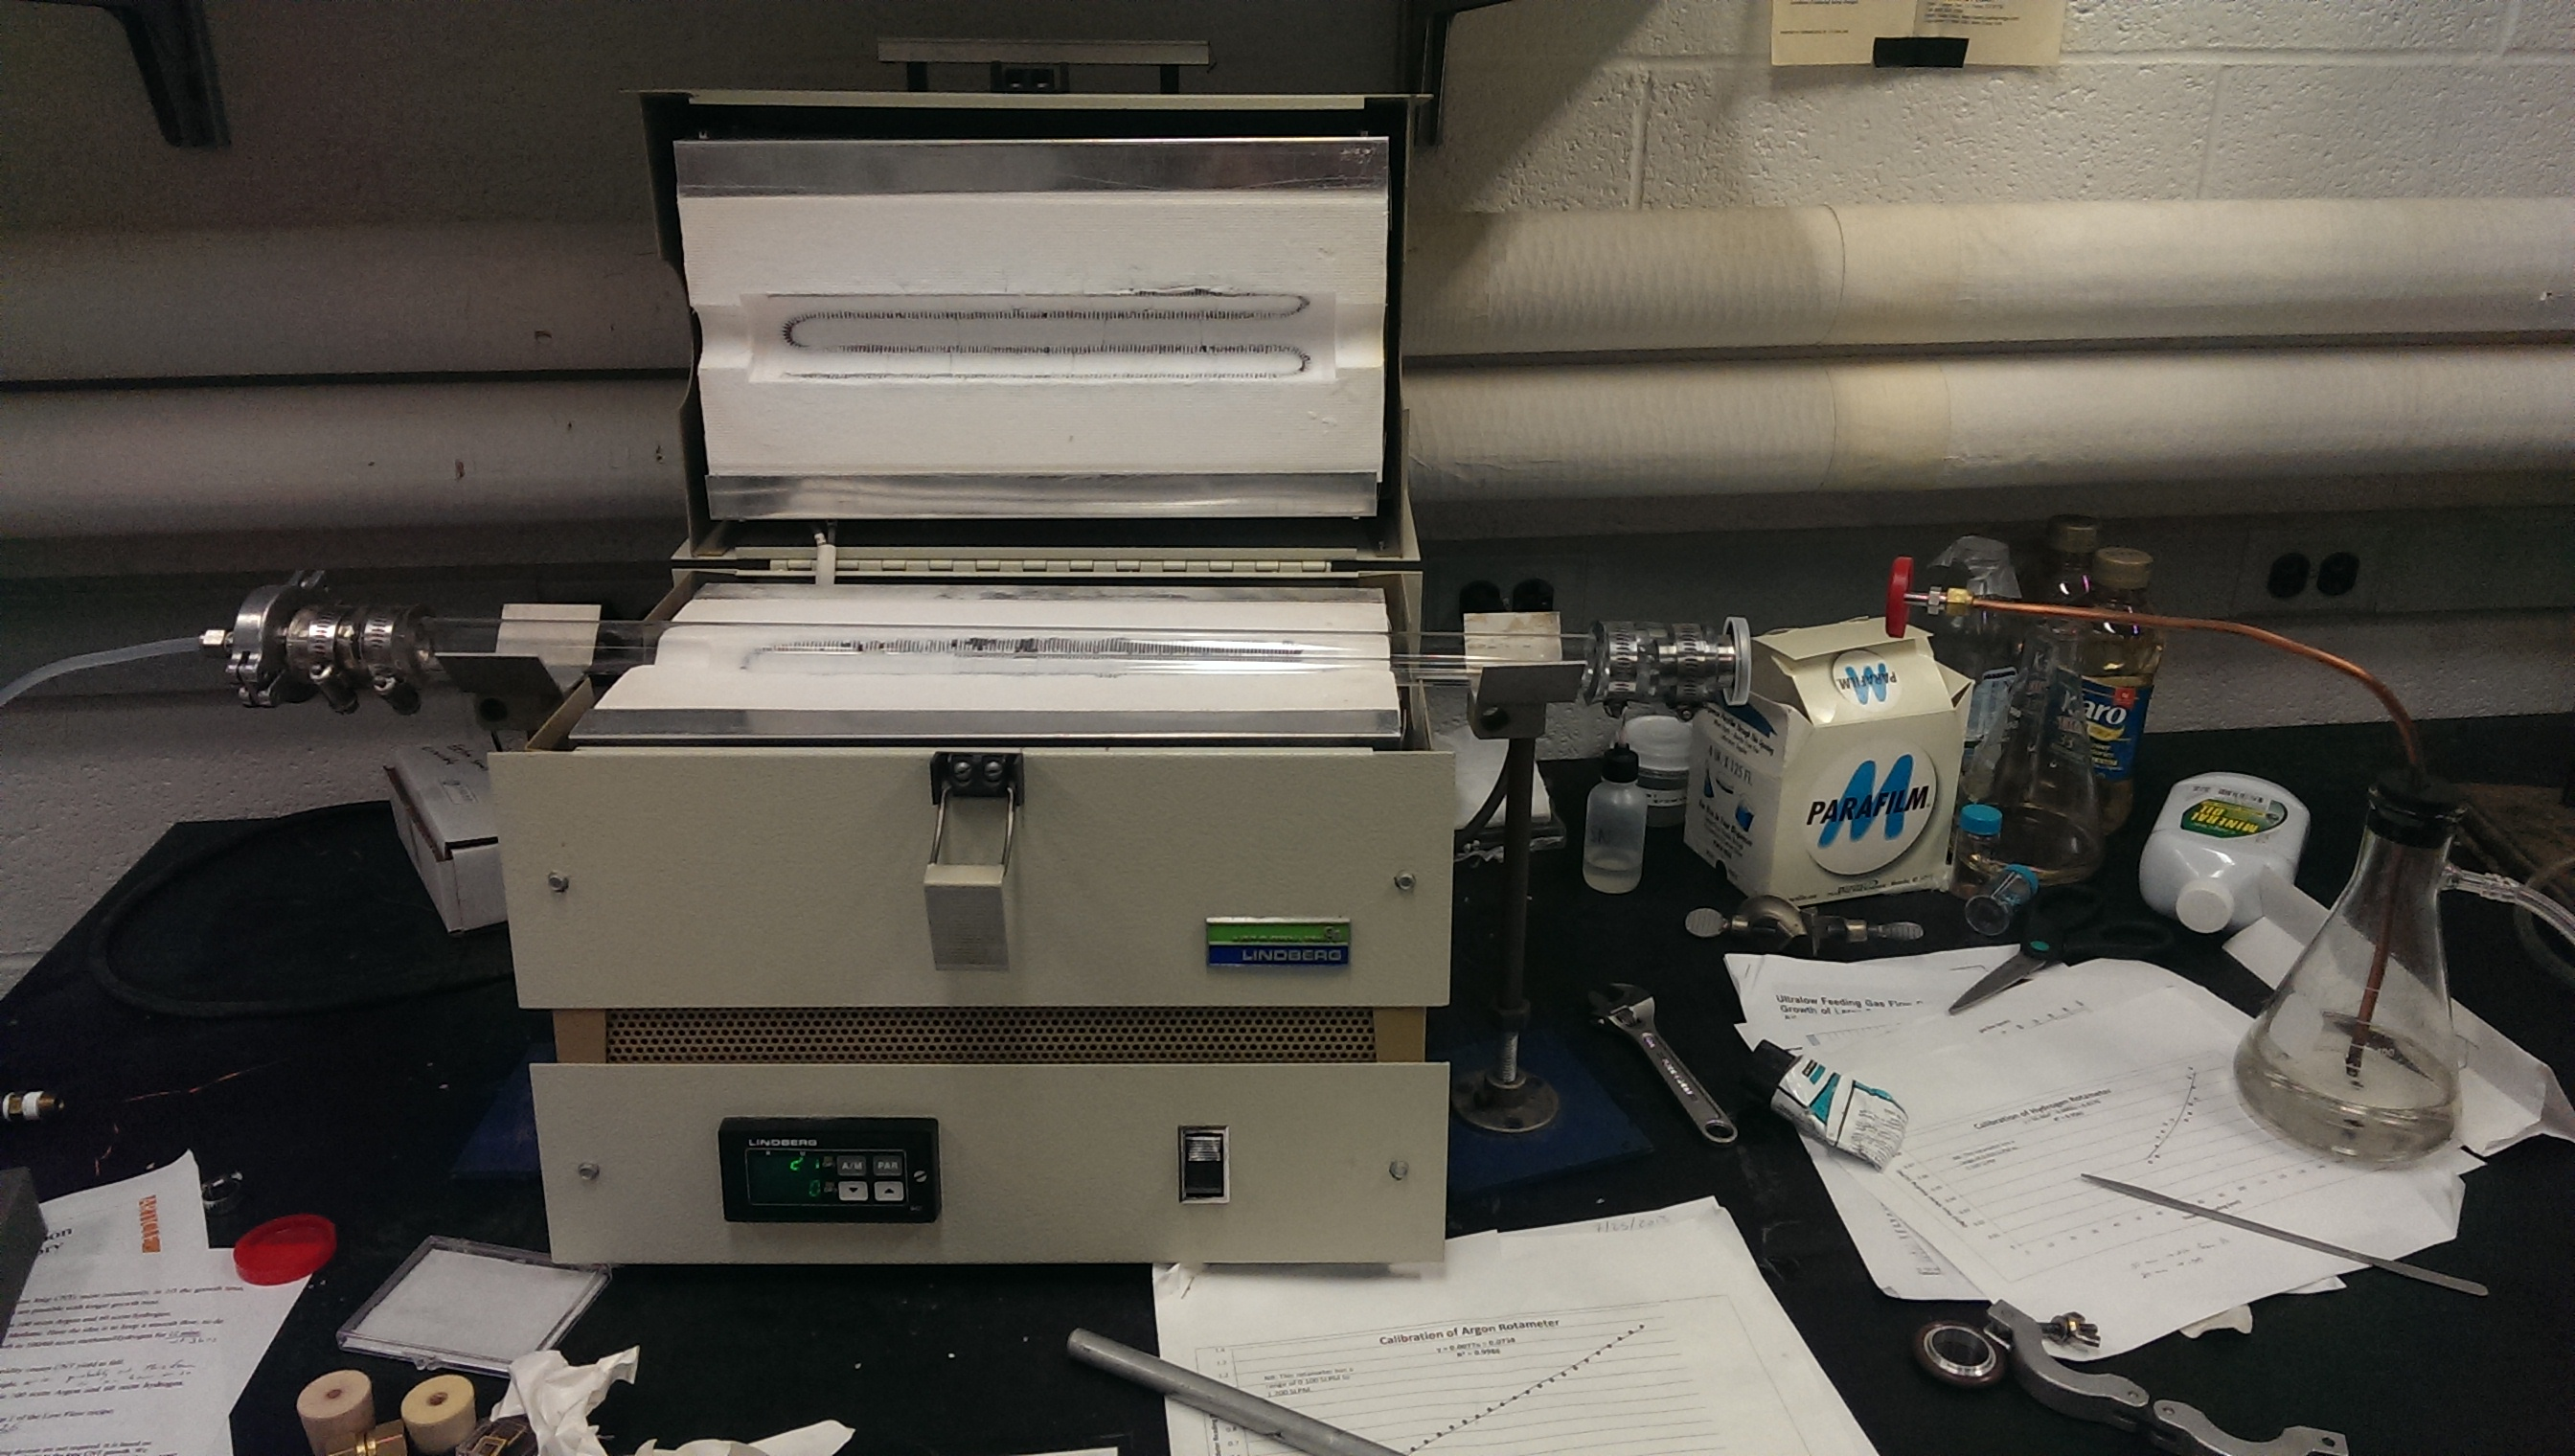
\includegraphics[width = 0.8\textwidth]{chapter3/furnace_setup.jpg}
    \caption{The tube furnace fitted with a 1" diameter quartz tube. The tube is sealed at both ends using 1" rubber tubing, cable clamps, and KF25 fittings. Gas flows from left to right in the picture. The gas flows out of the furnace into a mineral oil bubbler to keep hot hydrogen from reaching the air in the room. Gas then flows from the bubbler into the building exhaust.}
    \label{fig:furnace_setup}
\end{figure}

The gases used in the CVD process, argon, hydrogen, and methane, are fed into the furnace using a custom-made gas handling panel. This was originally constructed by Matt Oresky, a JHU undergraduate working in our lab with post-doc Atikur Rahman. The panel has three gas channels, each with its own analog flowmeter, needle valve, and on/off valve. A digital flowmeter placed at the right side of the panel reads the total flow of combined gas exiting the panel to the furnace. The gas handling panel can be see in Figure~\ref{fig:gas_panel}

\begin{figure}
    \centering
    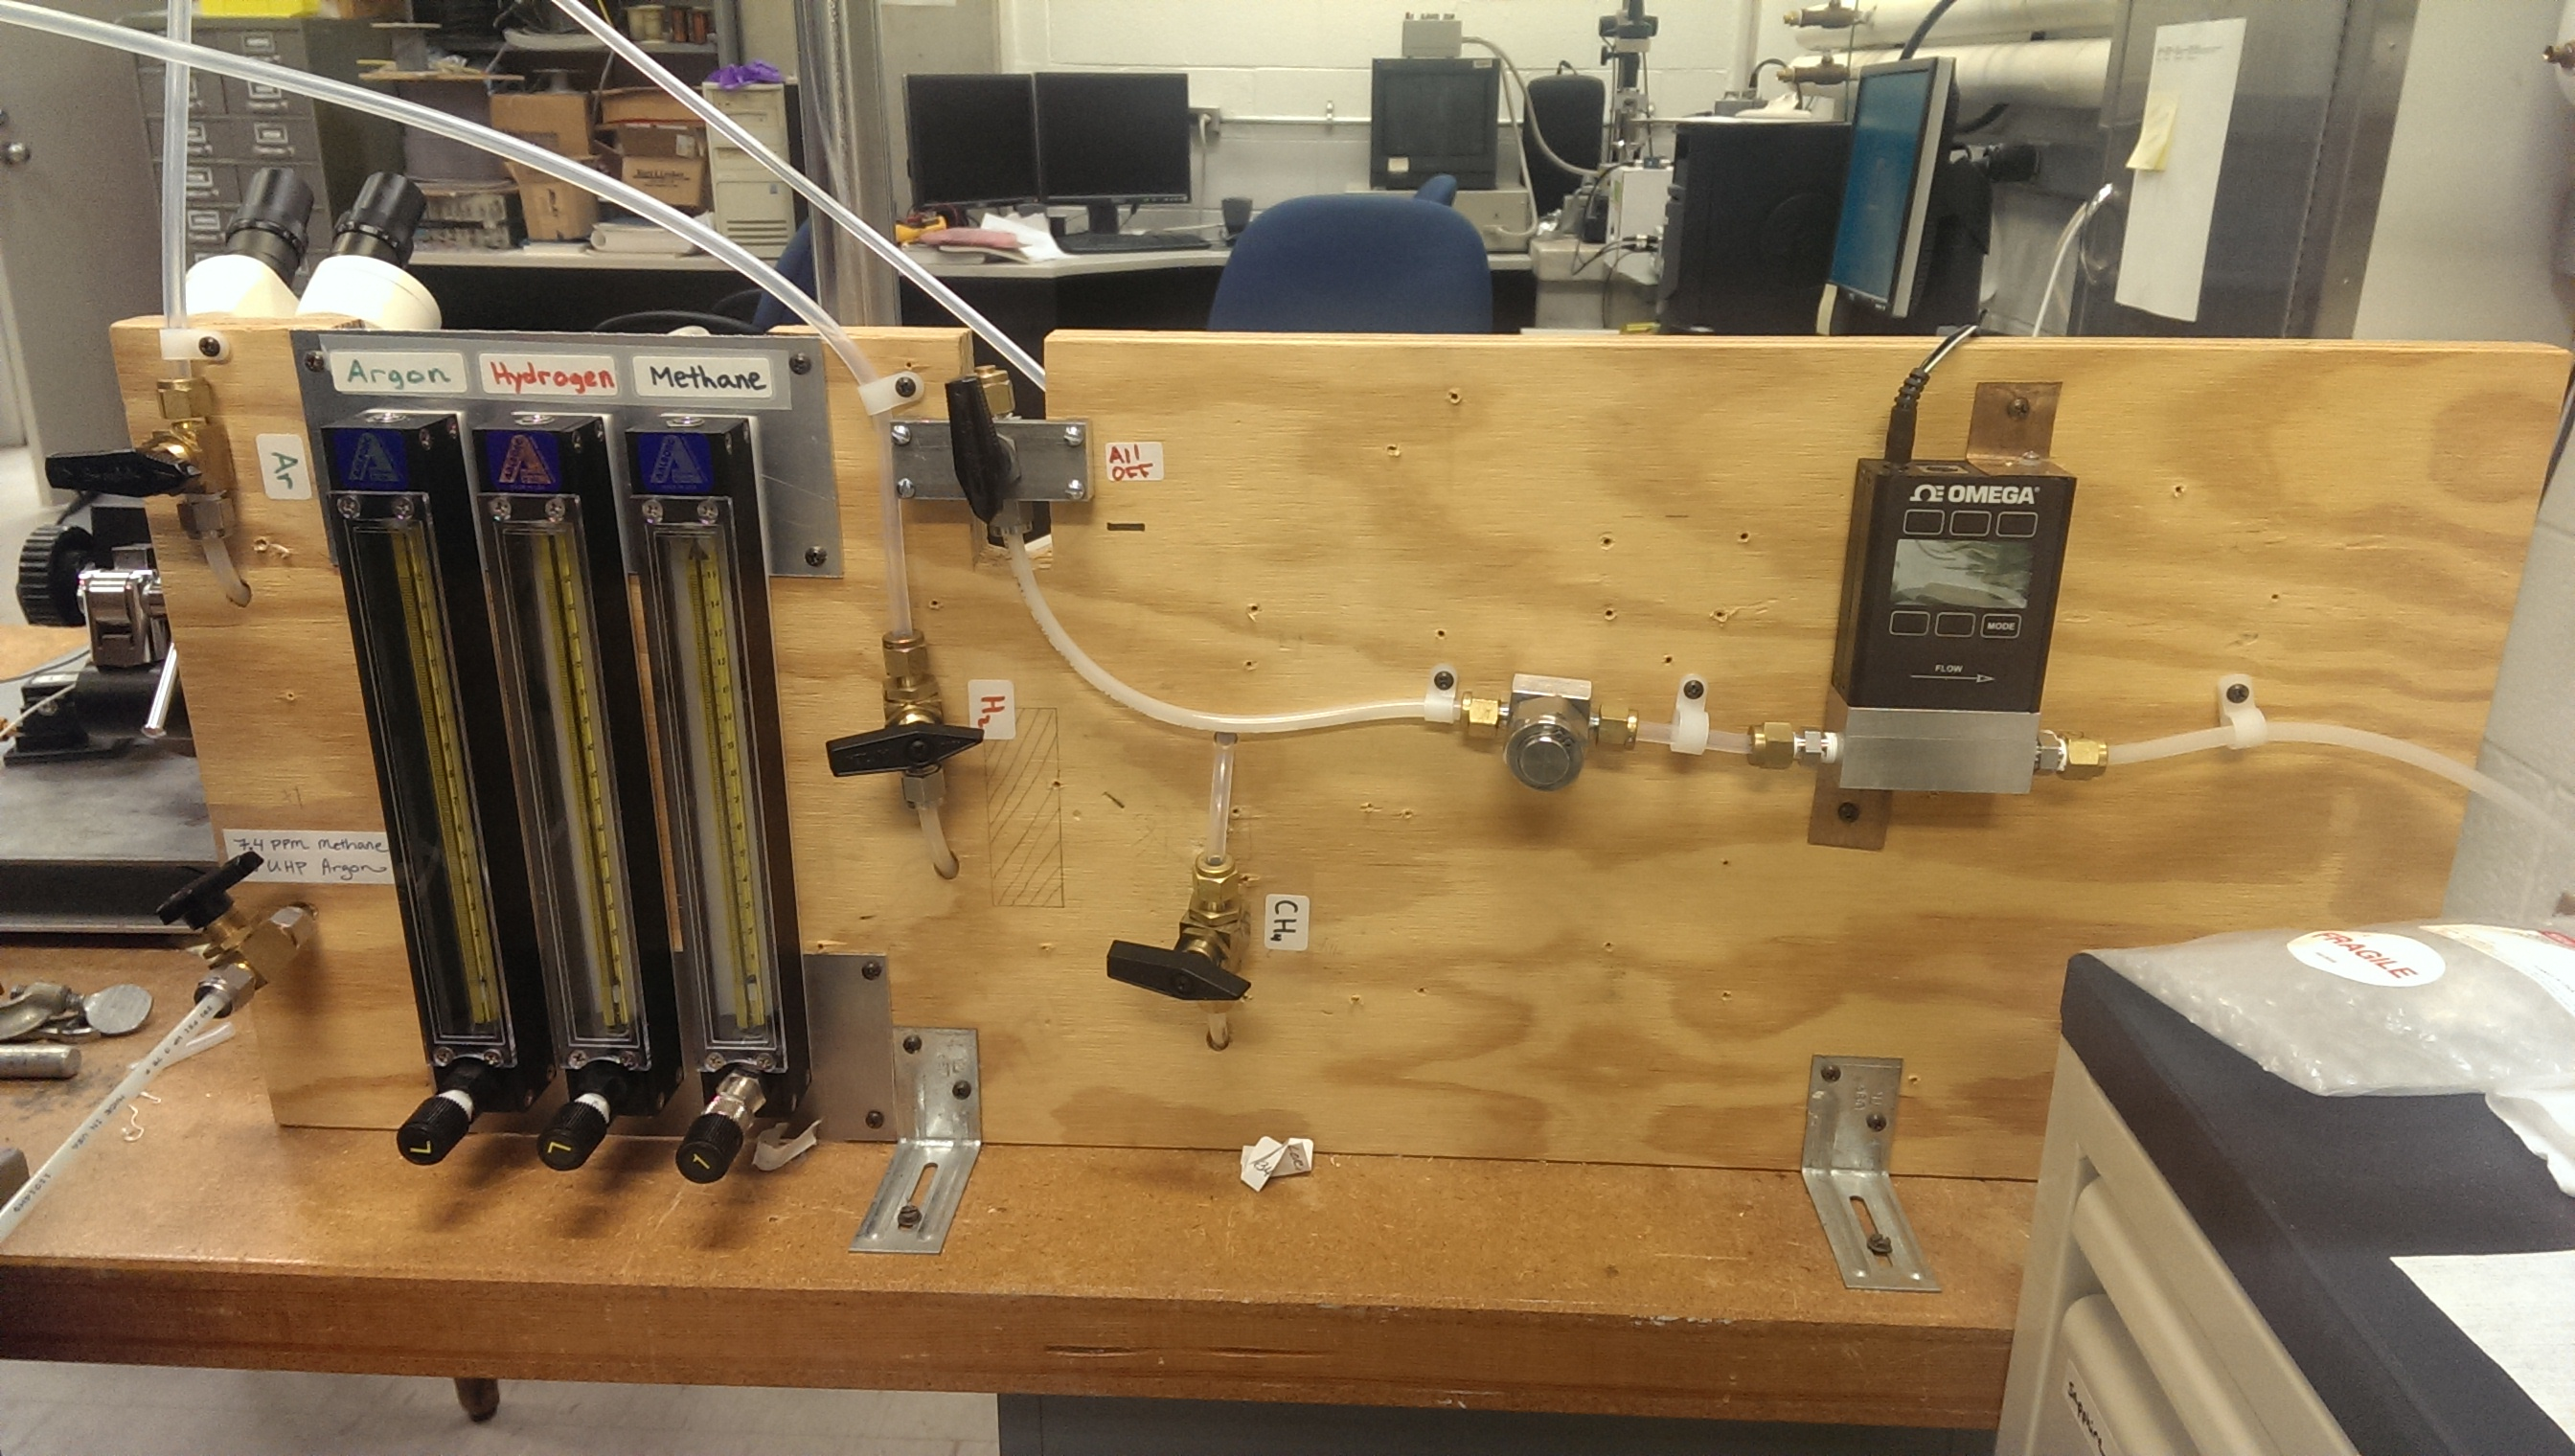
\includegraphics[width = 0.8\textwidth]{chapter3/gas_panel.jpg}
    \caption{The gas handling panel for our Lindberg tube furnace. Gas flow is from left to right.}
    \label{fig:gas_panel}
\end{figure}

The growth procedure begins with filling a ceramic crucible with the iron catalyst described in \ref{subsec:disperse_catalyst}. The catalyst should be spread in a thin layer across the bottom of the crucible, which is then loaded into the center of a 2-4 foot long quartz tube. The tube is sealed at each end, one side connected to the gas handling panel, and the other connected to the mineral oil filter and building exhaust. Our standard nanotube growth recipe is as follows: 

%can i remove the spacing from between these list items?
\begin{enumerate}
	\item Purge the tube by flowing \SI{2000}{\sccm} of Ar for 20 minutes
	\item Heat tube to \SI{1000}{\degreeCelsius} while flowing \SI{1000}{\sccm} Ar and \SI{200}{\sccm} \ce{H2}
	\item Flow \SI{2000}{\sccm} \ce{CH4} and \SI{200}{\sccm} \ce{H2} for 10 minutes.
	\item Set temperature to \SI{0}{\degreeCelsius} and let the furnace cool while flowing \SI{1000}{\sccm} Ar and \SI{200}{\sccm} \ce{H2}
\end{enumerate}

\noindent The actual nanotube growth occurs during the methane flow step. The \SI{200}{\sccm} \ce{H2} flow can be omitted, but it does seem to help promote nanotube growth. The flow rates do not need to be precise. Most nanotubes grow in the first few seconds of methane flow regardless of the flow rate. The Ar and \ce{H2} are simply to keep \ce{O2} and \ce{H2O} out of the tube. 

\subsection{Nanotube Placement}

After the CVD process, the nanotubes remain attached to the iron\slash alumina\slash molybdenum catalyst particles, which must be removed before depositing onto a silicon substrate. The nanotube\slash catalyst powder is first scraped from the ceramic crucible used in the tube furnace. The powder is then mixed with either dichloroethane or dichlorobenzne in a \SI{1}{\milli\gram} to \SI{10}{\milli\liter} ratio. Dichlorobenze has been found to leave less residue after deposition, but may promote more damage to nanotubes during sonication. Some attempts were made to use water along with the surfactant SDS. However, SDS turned out to be difficult to remove and no devices were made in this way.

To remove the catalyst particles from the nanotubes, the solution described above must be placed in an ultrasonic bath for 1-60 minutes. The amount of time needed varied a great deal depending on the equipment and solvent used. The goal of this step is to break up large pieces of catalyst, separate nanotube bundles, and break individual nanotubes away from their catalyst particles. Sonication can be stopped when no large pieces of catalyst\slash nanotube material are visible and the solution has a uniform black color. Leaving the solution in the sonicator for too much time will begin to break long nanotubes. 

When sonication is complete, the solution is transferred to a centrifuge. This step is intended to precipitate the loose catalyst particles from the solution, while leaving the much lighter nanotubes suspended. The centrifuge used in our lab runs at \SI{2200}{\rpm} and nanotube solutions are left inside for 5-10 minutes. Once the centrifuge stops, the precipitate is discarded and the supernate, containing the suspended nanotubes, is reserved. We also tested using a high-speed, air-powered centrifuge running at \SI{100000}{\rpm} to separate nanotubes and catalyst. This did lead to much better catalyst separation and cleaner results,.

Now the solution is ready for deposition on a silicon substrate. The substrates are typically pre-patterned with a set of reference markers placed by optical (\ref{subsec:optical}) or electron beam lithography (\ref{sec:ebeam_lith}). An example of a patterned substrate can be seen in Figure \ref{fig:markers}

\begin{figure}
    \centering
    \includegraphics[width = 0.8\textwidth]{chapter3/markers.eps}
    \caption{A \ce{Si}/\ce{SiO2} substrate with \SI{1}{\micro\meter} \ce{Au} markers. Left scale bar: \SI{100}{\micro\meter}. Right scale bar: \SI{20}{\micro\meter} }
    \label{fig:markers}
\end{figure}

\subsection{Conclusion}

Despite having some success fabricating devices using randomly dispersed nanotubes and EFM scans, the process was found to be too unreliable for frequent use. The main failure point was the preparation of nanotube solutions after growth. The concentrations varied significantly, often producing samples with dense nanotube coverage or no nanotubes found in the regions imaged. Additionally, the process of making a suspended nanotube solution is time consuming. Even those solutions with a useful concentration of nanotubes only remain fully suspended for less than 1 hour.

\section{Catalyst Island Growth}
\label{subsec:catalyst_island}

In 1998 \cite{Kong1998a}, it was discovered that the same type of catalyst used to grow nanotubes in powder form (Section \ref{subsec:disperse_catalyst}), could be suspended in solution, patterned, and used to grow nanotubes directly on silicon substrates. When paired with high melting point metals and optical lithography, nanotubes can be grown directly on patterned substrates in known locations. Devices prepared this way take just a fraction of the time to produce. 

\subsection{Catalyst} 

Many different types of catalyst particles can be used in the growth of carbon nanotubes. The ideal catalyst for patterned growth must be compatible with electron beam or optical lithography. Table \ref{table:catalysts} lists most of the catalysts tested in the Markovic lab. To test each catalyst, sputtered molybdenum leads were patterned using the mask aligner and Futurex NR9 resist. Catalyst islands were then patterned using electron beam lithography. Figure \ref{fig:catalyst_islands} shows an example of a substrate with Mo leads and catalyst islands.

\begin{figure}
	\centering
	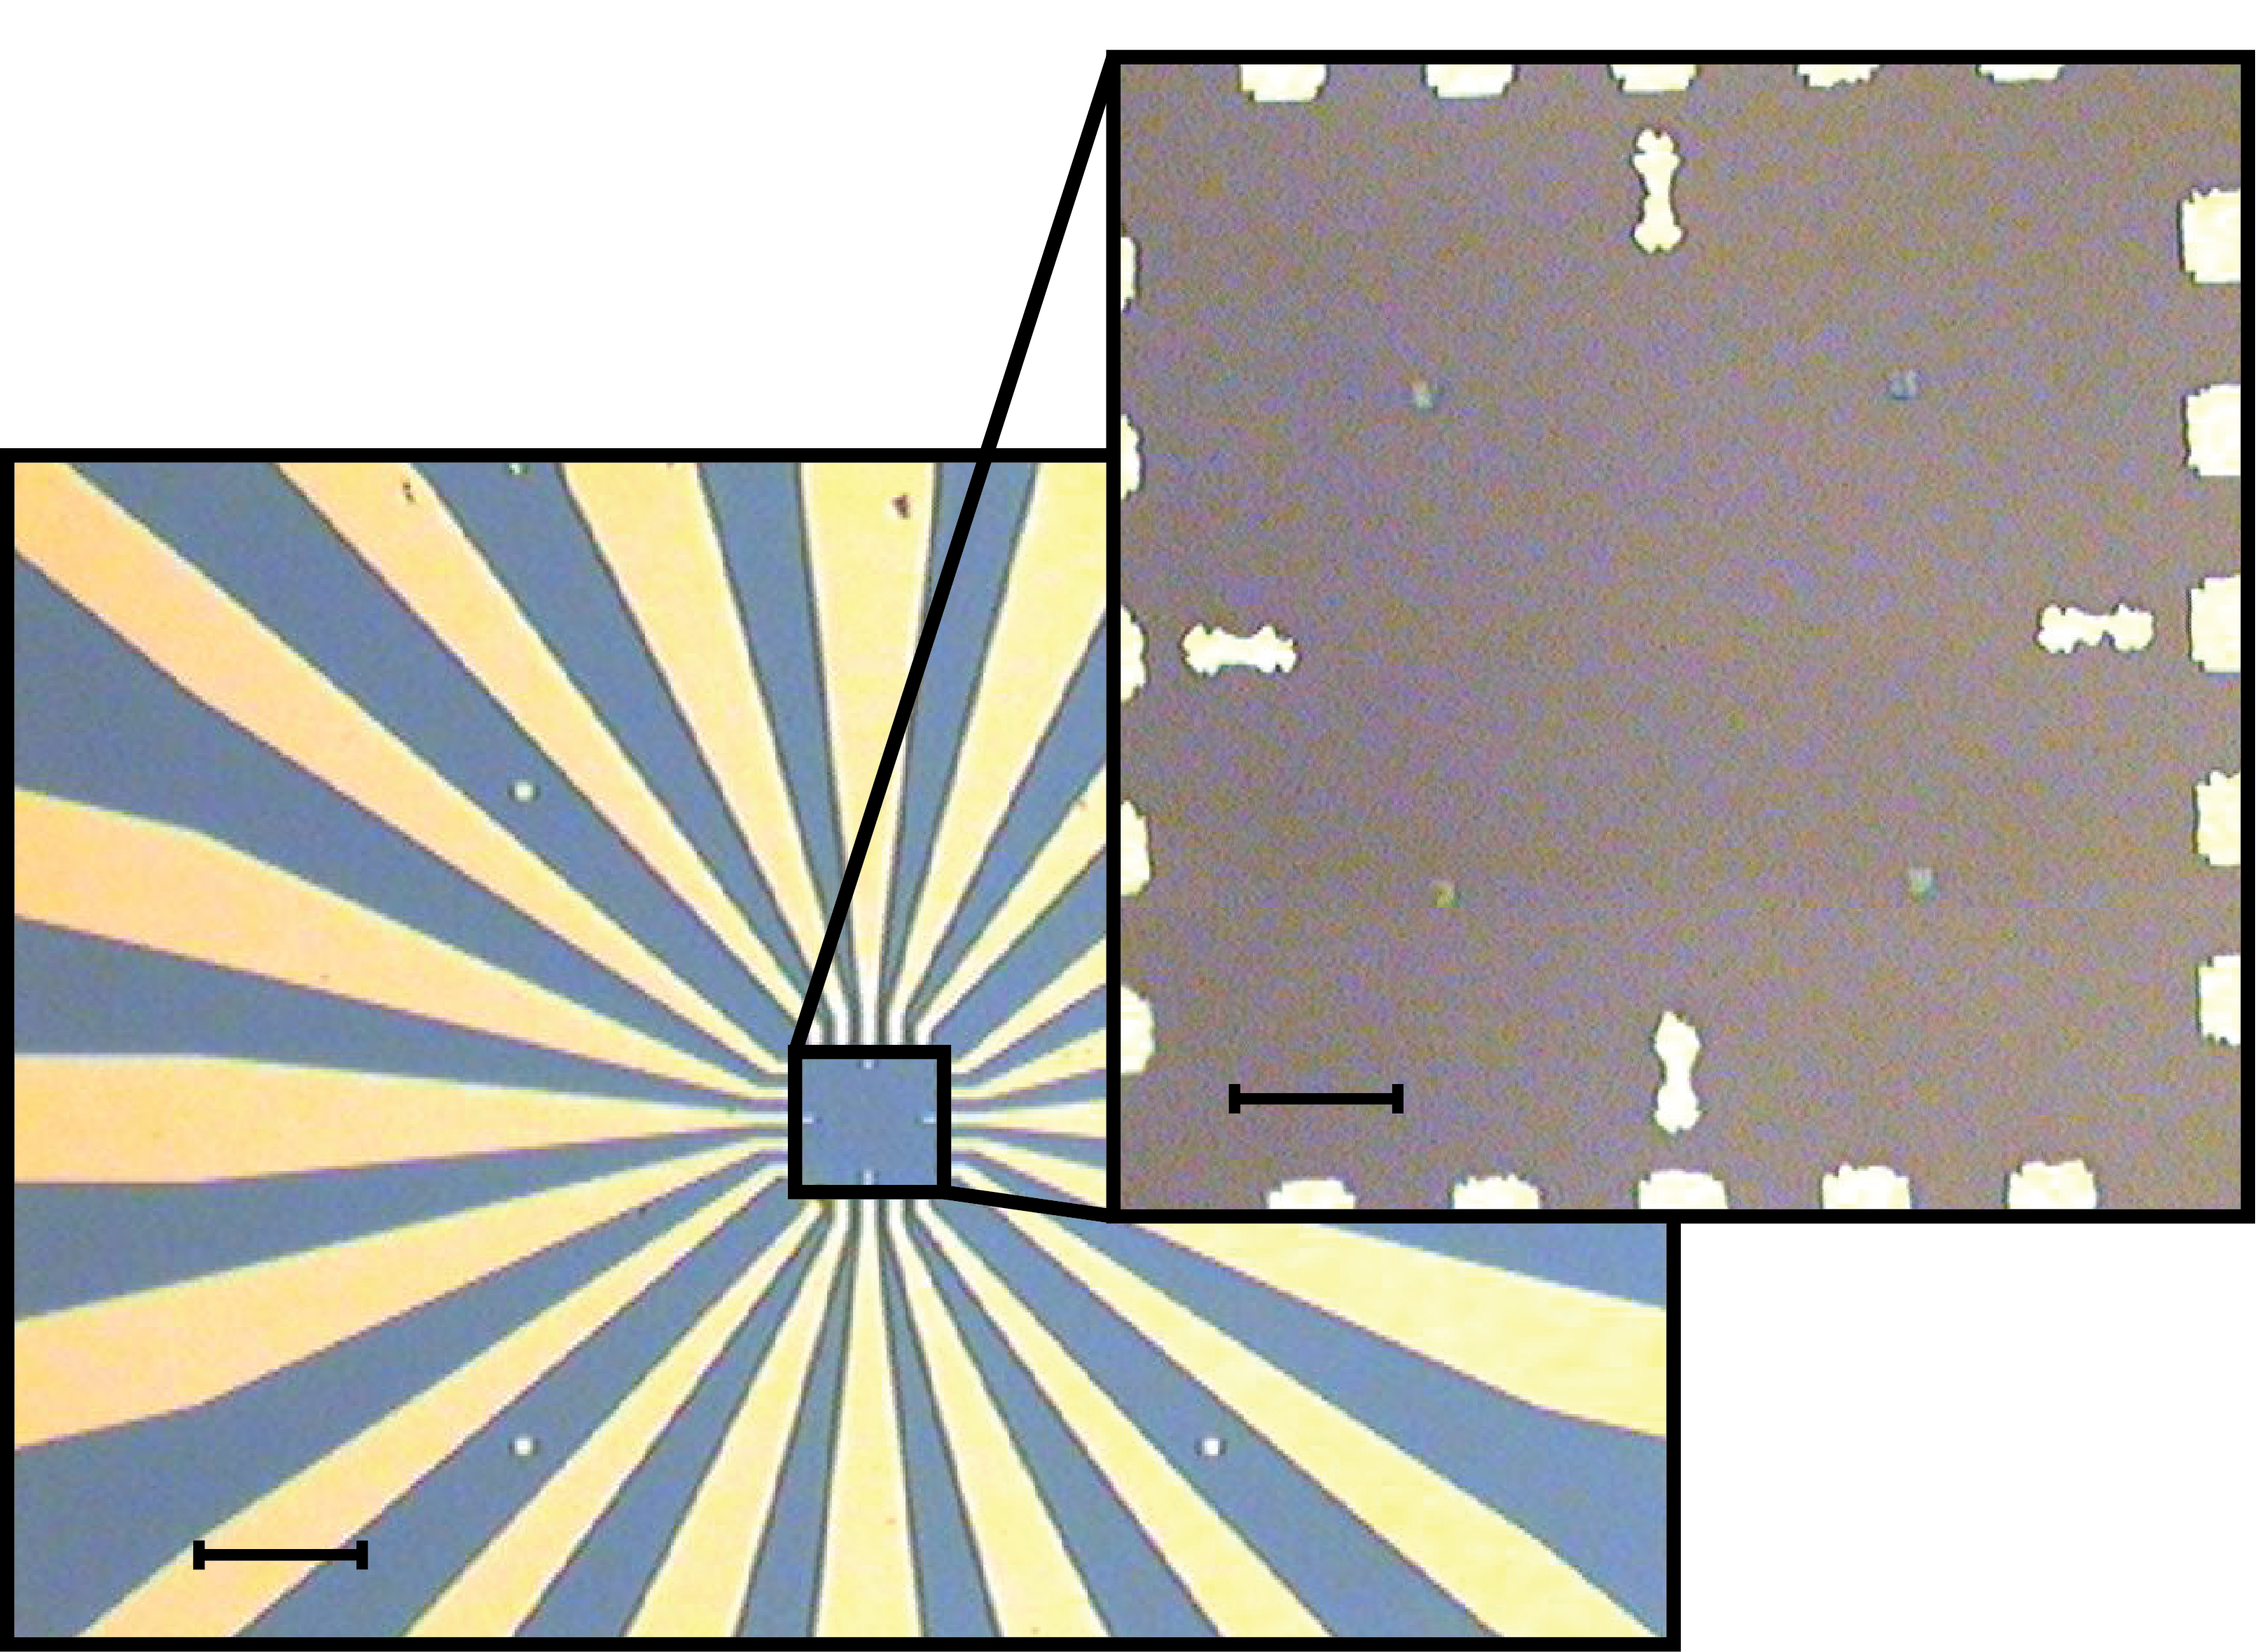
\includegraphics[width = 0.8\textwidth]{chapter3/catalyst_island.eps}
	\caption{A \ce{Si}/\ce{SiO2} substrate with \SI{3}{\micro\meter} catalyst islands and \ce{Mo} leads. Left scale bar: \SI{100}{\micro\meter}. Right scale bar: \SI{20}{\micro\meter} }
	\label{fig:catalyst_islands}
\end{figure}

\begin{table}
	\centering
	\caption{Patterned Catalysts}
    \begin{tabular}{| r | c || p{70mm} |}
    	\hline
    	\textbf{Catalyst} & \textbf{Suspended In} & \textbf{Results} \\ \hline
        Fe/Mo/alumina \cite{Kong1998} & Methanol & Easy to pattern. Liftoff difficult. Slowly attacks PMMA mask. Appeared to promote to gate leaks through the \ce{SiO2} layer. \\ \hline
        Fe/Mo/alumina \cite{Aurich2012} & IPA & Poor adhesion to substrate. \\ \hline
        Fe/Mo/alumina \cite{Ouellette2008} & DI water & Easy to pattern. Excellent adhesion. No gate leak problems. \\ \hline
        \ce{FeCl3} \cite{Hong2005} & DI water & Excellent adhesion to substrate. Not compatible with PMMA mask. Left substrate entirely covered in catalyst. May work well with PDMS stamp. \\ \hline
        thermally evaporated Fe \cite{Biercuk2004, Kang2007} & None & Very easy to pattern. Liftoff is clean. Difficult to control the thickness below \SI{1}{\nano\meter} as required. \\ \hline
    \end{tabular}
    \label{table:catalysts}
\end{table}

All of the devices discussed in this thesis were produced using the Fe\slash Mo\slash alumina catalyst suspended in water. The islands were patterned using electron beam lithography. Catalyst is deposited in the following way:

\begin{enumerate}
	\item Add the powder catalyst from Table \ref{table:powder_catalyst} to \SI{15}{\milli\liter} of DI water and stir for 12 hours
	\item Sonicate the solution for 30 minutes
	\item Cover the sample in catalyst solution for 30 minutes
	\item Dry with \ce{N2} gun
	\item Liftoff by sonicating in acetone for 5 minutes, soaking in a clean acetone for 5 minutes, followed by an isopropanol rinse for 1 minute and a DI water rinse for 1 minute
\end{enumerate}

Depositing the catalyst islands in a reproducible way proved to be the most difficult step in the fabrication of nanotube samples. It is suspected that baking the catalyst on a hot plate to dry the solution leads directly to gate leaks in the \ce{SiO2} layers and later device failure. Thus, there is no baking step in the deposition of our catalyst islands.

\subsection{Growth}
\label{subsubsec:substrate_cvd}

The recipe for on-substrate growth of nanotubes used in this thesis is very similar to the growth recipe for powder catalyst discussed in Section \ref{subsubsec:powder_cvd}. This recipe was developed over the course of several years from many points of reference \cite{Kong1998, Kong1998a, Dirks2010, Huang2003, Huang2004, Zhang2013, Hong2005} and a my own notes. The recipe is optimized for the 1 inch Lindberg tube furnace as seen in Figures \ref{fig:furnace_setup} and \ref{fig:gas_panel}. Most samples are placed in a smaller \SI{1}{\centi\meter} diameter, 1 foot long quartz tube, then placed in the larger 1 inch diameter quartz tube. This was done to make the samples easier to load into the 1" tube, as well as to reduce turbulence in the gas flow across the sample \cite{Hong2005}. 

The standard nanotube growth recipe used in this work is below:

\begin{enumerate}
	\item Purge the tube by flowing \SI{2000}{\sccm} of Ar for 20 minutes
	\item Heat the tube to \SI{250}{\degreeCelsius} while flowing \SI{300}{\sccm} Ar and \SI{150}{\sccm} \ce{H2}
	\item Wait for at least 1 hour
	\item Heat the tube to \SI{700}{\degreeCelsius} while flowing \SI{300}{\sccm} Ar and \SI{150}{\sccm} \ce{H2}
	\item Wait for 10 minutes
	\item Heat tube to \SI{950}{\degreeCelsius} while flowing \SI{300}{\sccm} Ar and \SI{150}{\sccm} \ce{H2}
	\item Wait for the temperature to stabilize
	\item Flow \SI{700}{\sccm} \ce{CH4} and \SI{150}{\sccm} \ce{H2} for 10-15 minutes
	\item Set temperature to \SI{0}{\degreeCelsius} and let the furnace cool while flowing \SI{300}{\sccm} Ar and \SI{150}{\sccm} \ce{H2}
\end{enumerate}

In almost every case this recipe has grown nanotubes successfully. Steps 2 and 3 are included to remove water vapor from the air that might have collected inside the quartz tube on humid days \cite{Dirks2010}. Steps 4 and 5 are meant to remove iron oxide from the iron nanoparticles that make up the catalyst. 

The most common point of failure has been related to the patterned molybdenum leads on the substrate. Molybdenum oxidizes rapidly at high temperatures. Therefore, any oxygen contamination in the tube during the growth process will form a \ce{MoO} layer that is then quickly removed by reacting with the high temperature \ce{H2} flow. This process repeats and can lead to the Mo leads being entirely etched away. Additionally, it has been found that opening the furnace too soon during cooling can lead to the Mo leads peeling off of the substrate. This appears to be caused by some super-heating due to IR radiation reflecting off of the surfaces of the sample and quartz tube. It is a strange phenomenon that is avoided by allowing the furnace to cool to less than \SI{300}{\degreeCelsius} before opening the lid. These problems could also be solved by using a different high temperature metal such as a W/Pt bilayer, common in many other nanotube projects. Molybdenum was chosen for this work because it is easy to sputter and much more affordable.

\subsection{Conclusion}

Growing nanotubes from catalyst islands near predefined leads and markers offers a huge improvement over the method of random dispersion. Nanotubes produced with this method are longer, cleaner, and easier to locate. These improvements, along with the ability to produce many more samples in much less time, made this method the obvious choice for device fabrication.

\section{Imaging Nanotubes}
\label{subsubsec:imaging_disperse}

Nanotubes on a \ce{SiO2} surface can be located in a number of ways. This section will review a number of different methods, focusing on improvements made in the course of this thesis work.

\subsection{Atomic Force Microscopy}

With nanotubes that have been drop cast onto the surface, the standard method is to locate the tubes relative to the predefined markers using a tapping mode atomic force microscope (AFM). An example of an image created this way is seen in Figure \ref{fig:cnt_au_markers}. 

\begin{figure}
	\centering
	\includegraphics[width = 0.8\textwidth]{chapter3/cnt_au_markers.eps}
	\caption{A composite image made from several AFM height measurements of a sample with nanotubes dispersed over a  substrate with \SI{1.5}{\micro\meter} gold markers. The scale bar is \SI{10}{\micro\meter}.}
	\label{fig:cnt_au_markers}
\end{figure}

This method is very reliable, but extremely time consuming. In order to resolve nanotubes, as well as the predefined markers in the image, AFM scan sizes must be limited to \SI{25}{\square\micro\meter}. Each of these scans takes 30 minutes and many scans are needed to fully image one patterned substrate. Looking closely at Figure \ref{fig:cnt_au_markers}, there are 12 scans covering less than half the substrate. Due to vibrational noise and piezo limits, some images are slightly warped. Stitching the images together is time consuming and inaccurate.

\subsection{Electric Force Microscopy}

The Digital Instruments Nanoscope 3 used in our lab is also capable of making electric force microscope (EFM) measurements. An EFM image is made by first measuring the height across the sample in standard tapping mode, then using that height data to run a second 'interleave' scan at a fixed height with a bias voltage applied between the tip and sample. By holding the tip at a fixed height, van der Waals interactions between the tip and sample are constant and the only force measured is the electrostatic force from the applied bias voltage. Contrast in the resulting images is related to the different conductivities of the objects on the sample \cite{Bockrath2002}. Thus, conducting (and semiconducting) nanotubes have a high contrast against the insulating \ce{SiO2} substrate. An example of this type of image is shown in Figure \ref{fig:cnt_efm}

\begin{figure}
	\centering
	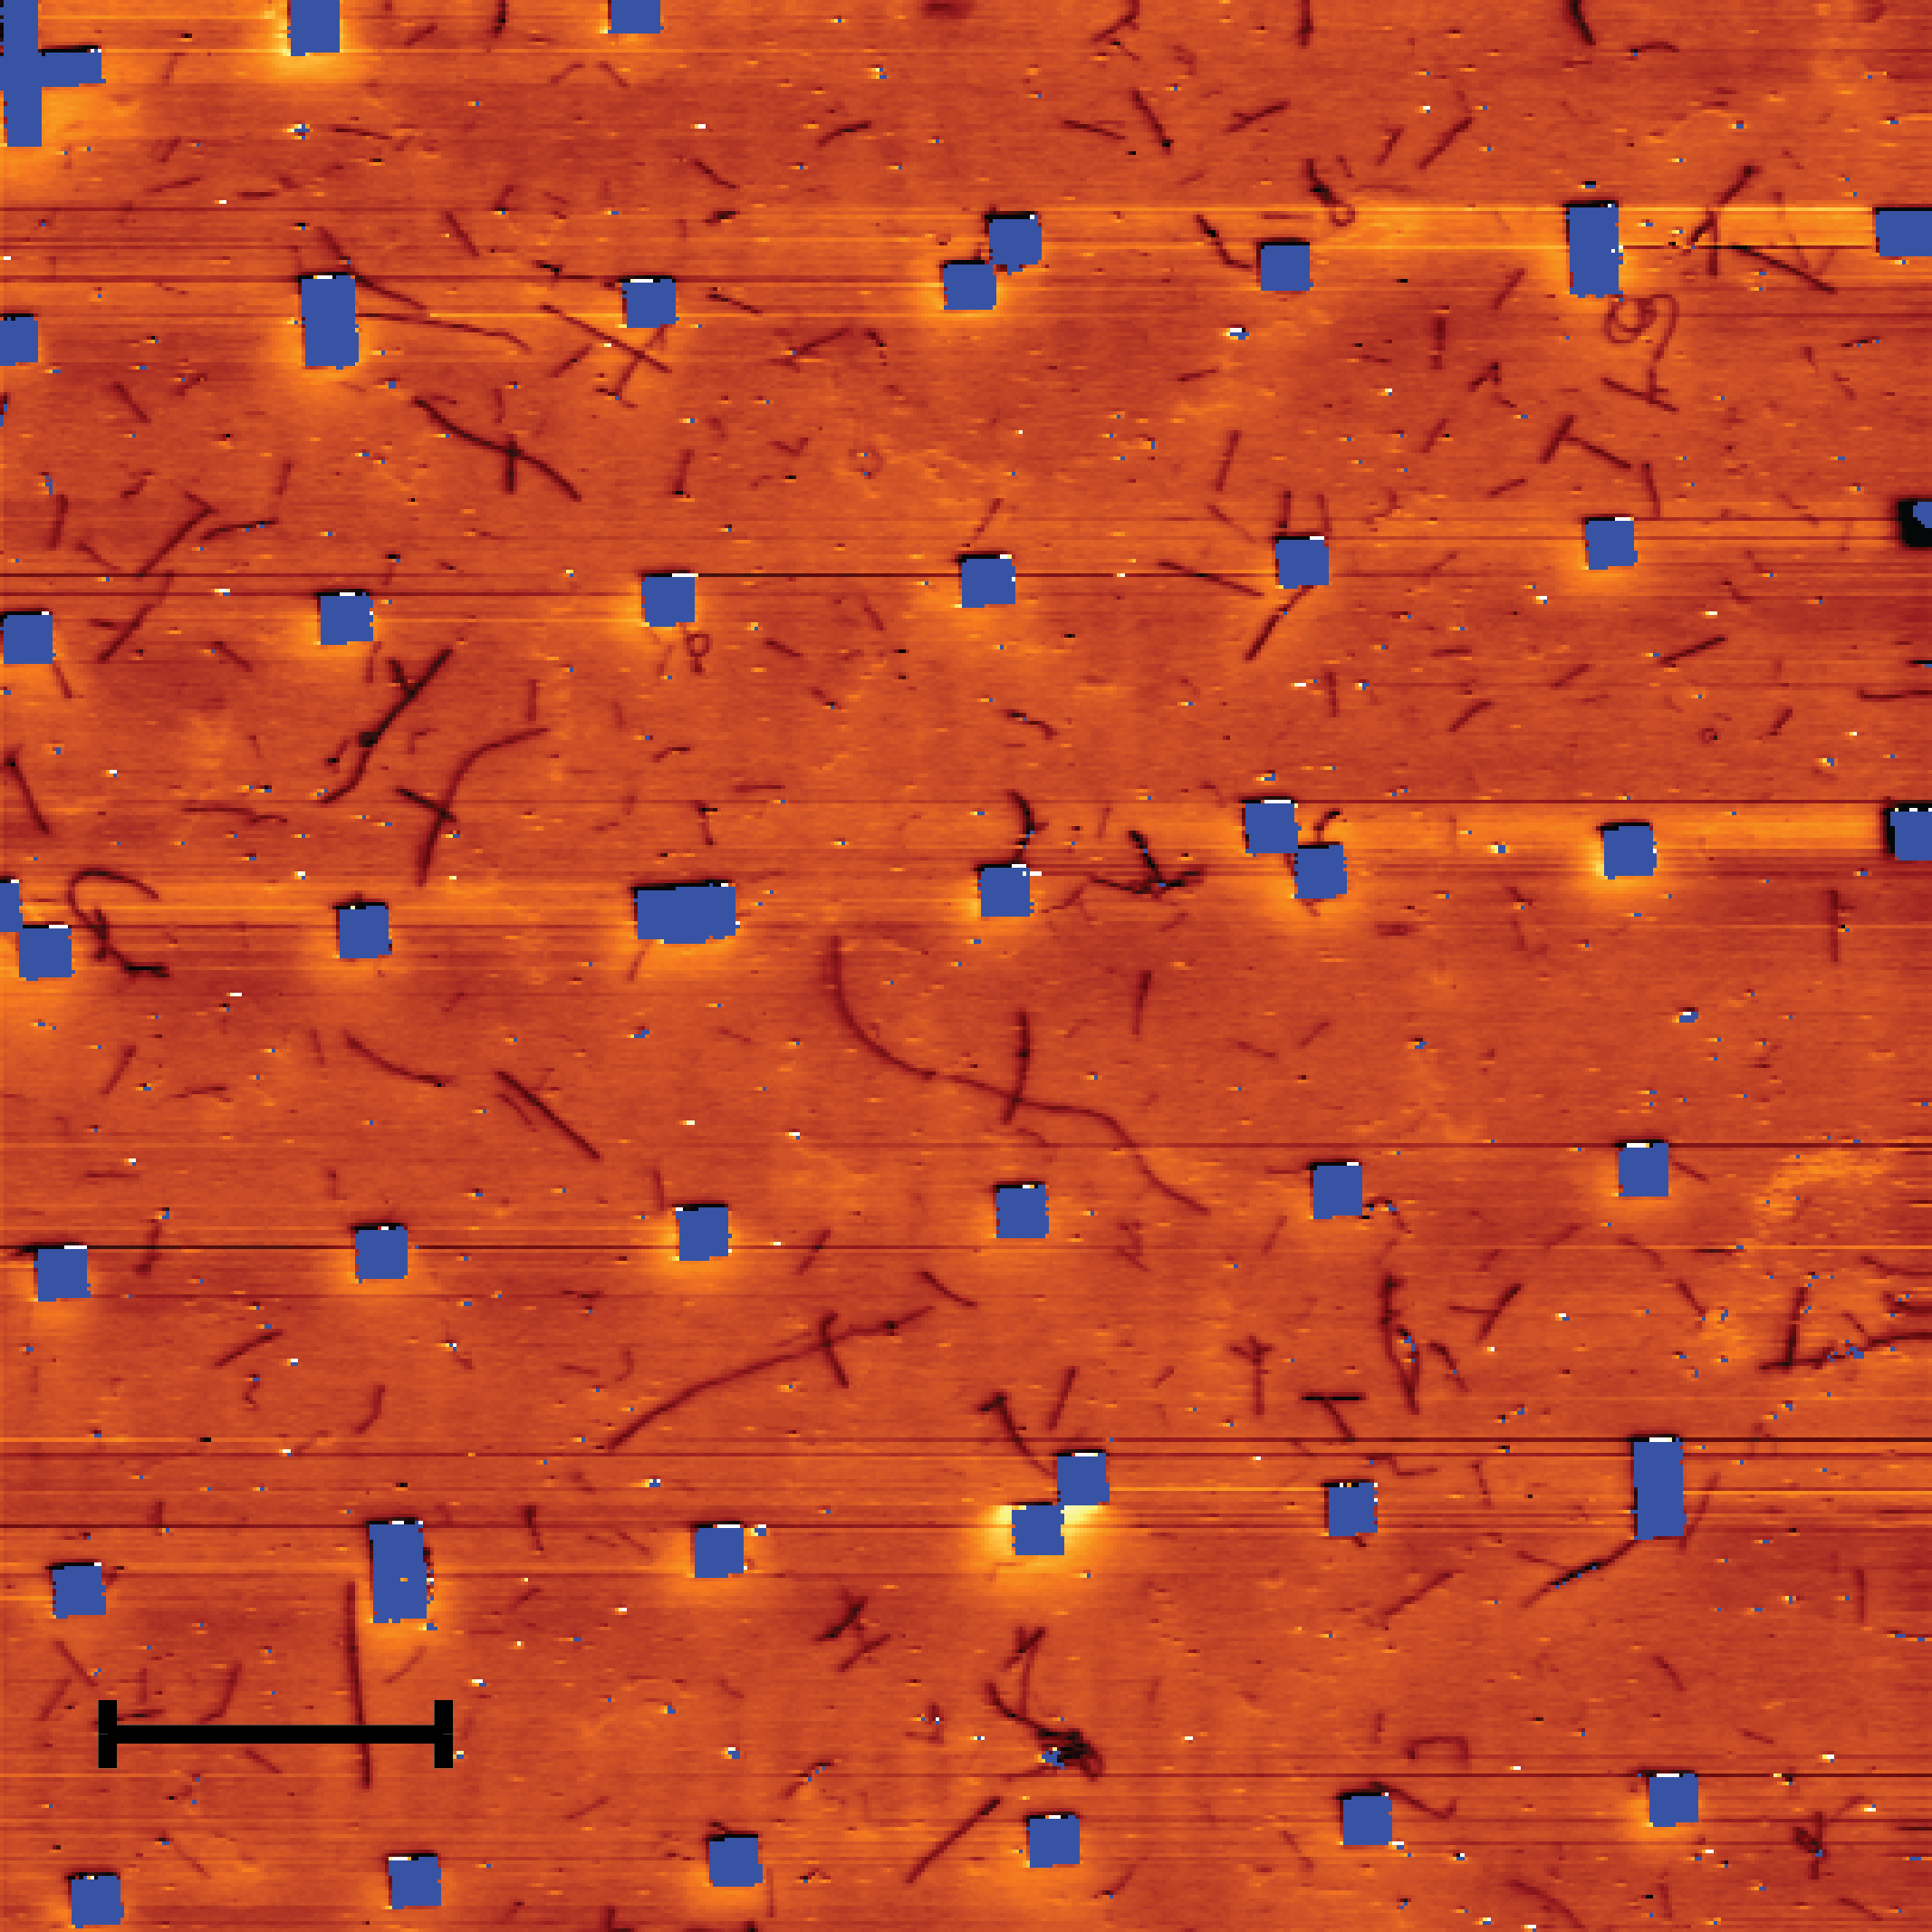
\includegraphics[width = 0.8\textwidth]{chapter3/cnt_efm.eps}
	\caption{An EFM image of nanotubes dispersed over a substrate with \SI{1.5}{\micro\meter} gold markers. The markers have been automatically located using the height data and highlighted in blue on the EFM image. The scale bar is \SI{10}{\micro\meter}.}
	\label{fig:cnt_efm}
\end{figure}

An entire patterned substrate can be scanned using this method in about 1 hour. The scan size can be increased up to \SI{75}{\square\micro\meter} due to the false contrast provided by the large electrostatic forces between the nanotubes and the tip. Rather than appearing as \SI{1}{\nano\meter} in diameter, the tubes appear in the EFM image to be about 100 times their real diameter. This was a notable improvement over locating nanotubes using AFM height scans alone. Comparing Figure \ref{fig:cnt_au_markers} and Figure \ref{fig:cnt_efm}, it is clear the EFM image is far more useful in locating nanotubes.

\subsection{EFM Through PMMA}

All of the same techniques from Section \ref{subsubsec:imaging_disperse} can be applied to imaging nanotubes grown from patterned catalyst islands. However, because the substrates are not covered in closely spaced markers, it was found that tapping mode AFM height scans were not useful. Scans could only cover a small part of the sample and the resulting images were difficult to orient.

Using electric force microscopy (EFM) made it possible to scan the entire region of interest on the sample in one measurement. An example of this type of scan is shown in Figure \ref{fig:efm_islands}a. As can be seen in that figure, it was difficult for the AFM tip to avoid crashing into the catalyst islands during the EFM sweep. The catalyst islands are several hundred nanometers in height while the other features on the substrate are less than \SI{10}{\nano\meter}. Such height differences make large area scans difficult in tapping mode. This problem can be avoided by coating the sample in PMMA before scanning with the EFM, as seen in Figure \ref{fig:efm_islands}b. The PMMA coating smooths the height differences between the substrate and catalyst islands, without compromising the contrast between the insulating substrate and conducting nanotubes. The idea was adopted from a 2007 paper in which the authors attempted to locate nanotubes suspended in a PMMA layer in three dimensions \cite{Jespersen2007}.

\begin{figure}
	\centering
	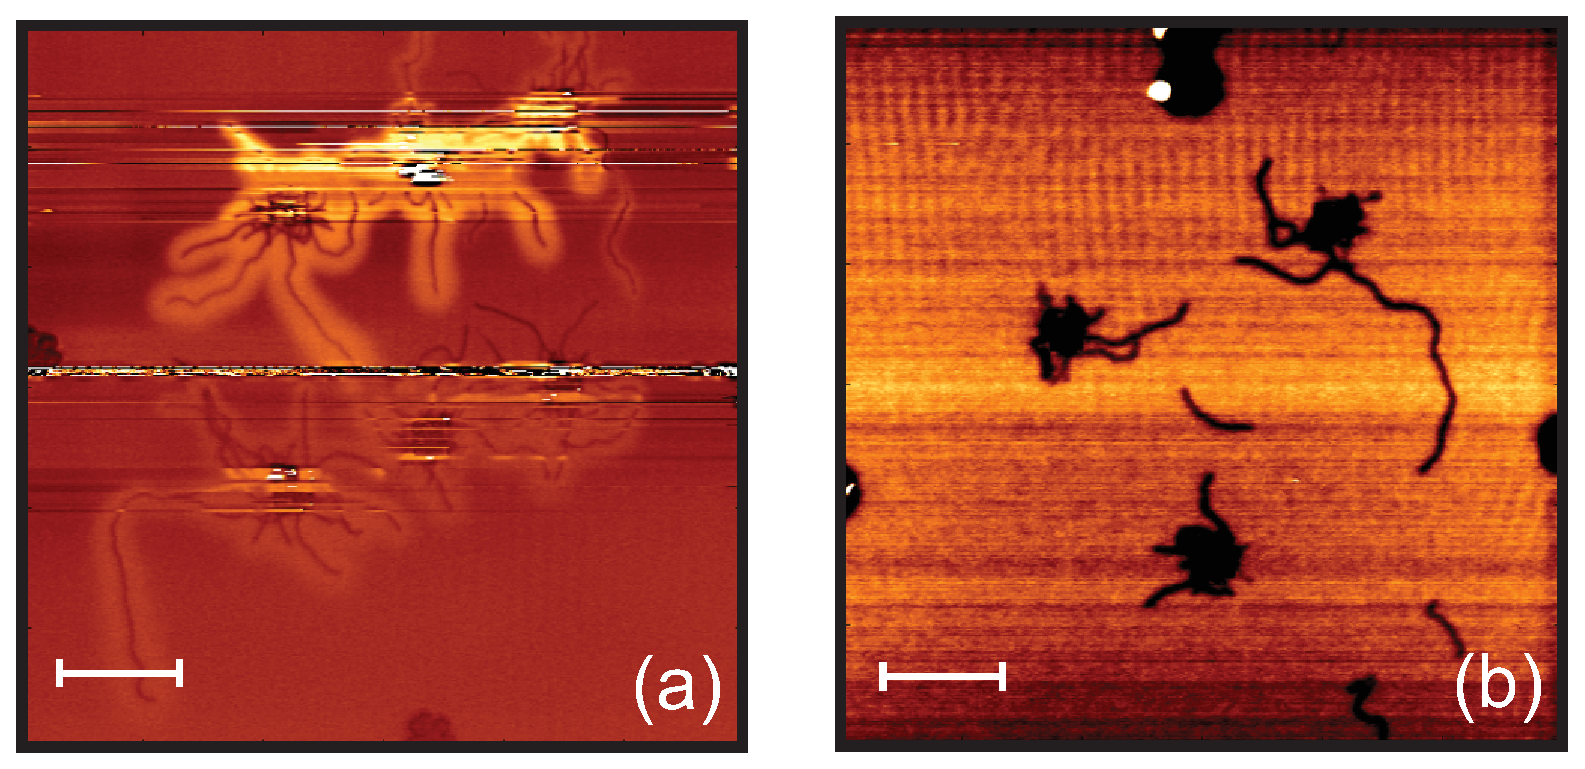
\includegraphics[width = 1.0\textwidth]{chapter3/efm_islands.eps}
	\caption{(a) Frequency data collected from an EFM scan of a catalyst island sample after nanotube growth. (b) Frequency data collected from an EFM scan of a similar sample. Prior to the scan this sample was coated with a \SI{250}{\nano\meter} PMMA layer. Both scale bars are \SI{10}{\micro\meter}. }
	\label{fig:efm_islands}
\end{figure}

\subsection{Scanning Electron Microscopy}

In 2002, a paper \cite{Brintlinger2002} was published illustrating that a scanning electron microscope (SEM), operating at a low accelerating potential could provide a similar type of false contrast image as produced by the EFM. The insulating substrate tends to collect charge from the electron beam, while the conducting nanotubes do not. This produces an image in which the nanotubes appear as bright lines about 100 times their actual diameter. An example of this is seen in Figure \ref{fig:sem_islands}. 

\begin{figure}
	\centering
	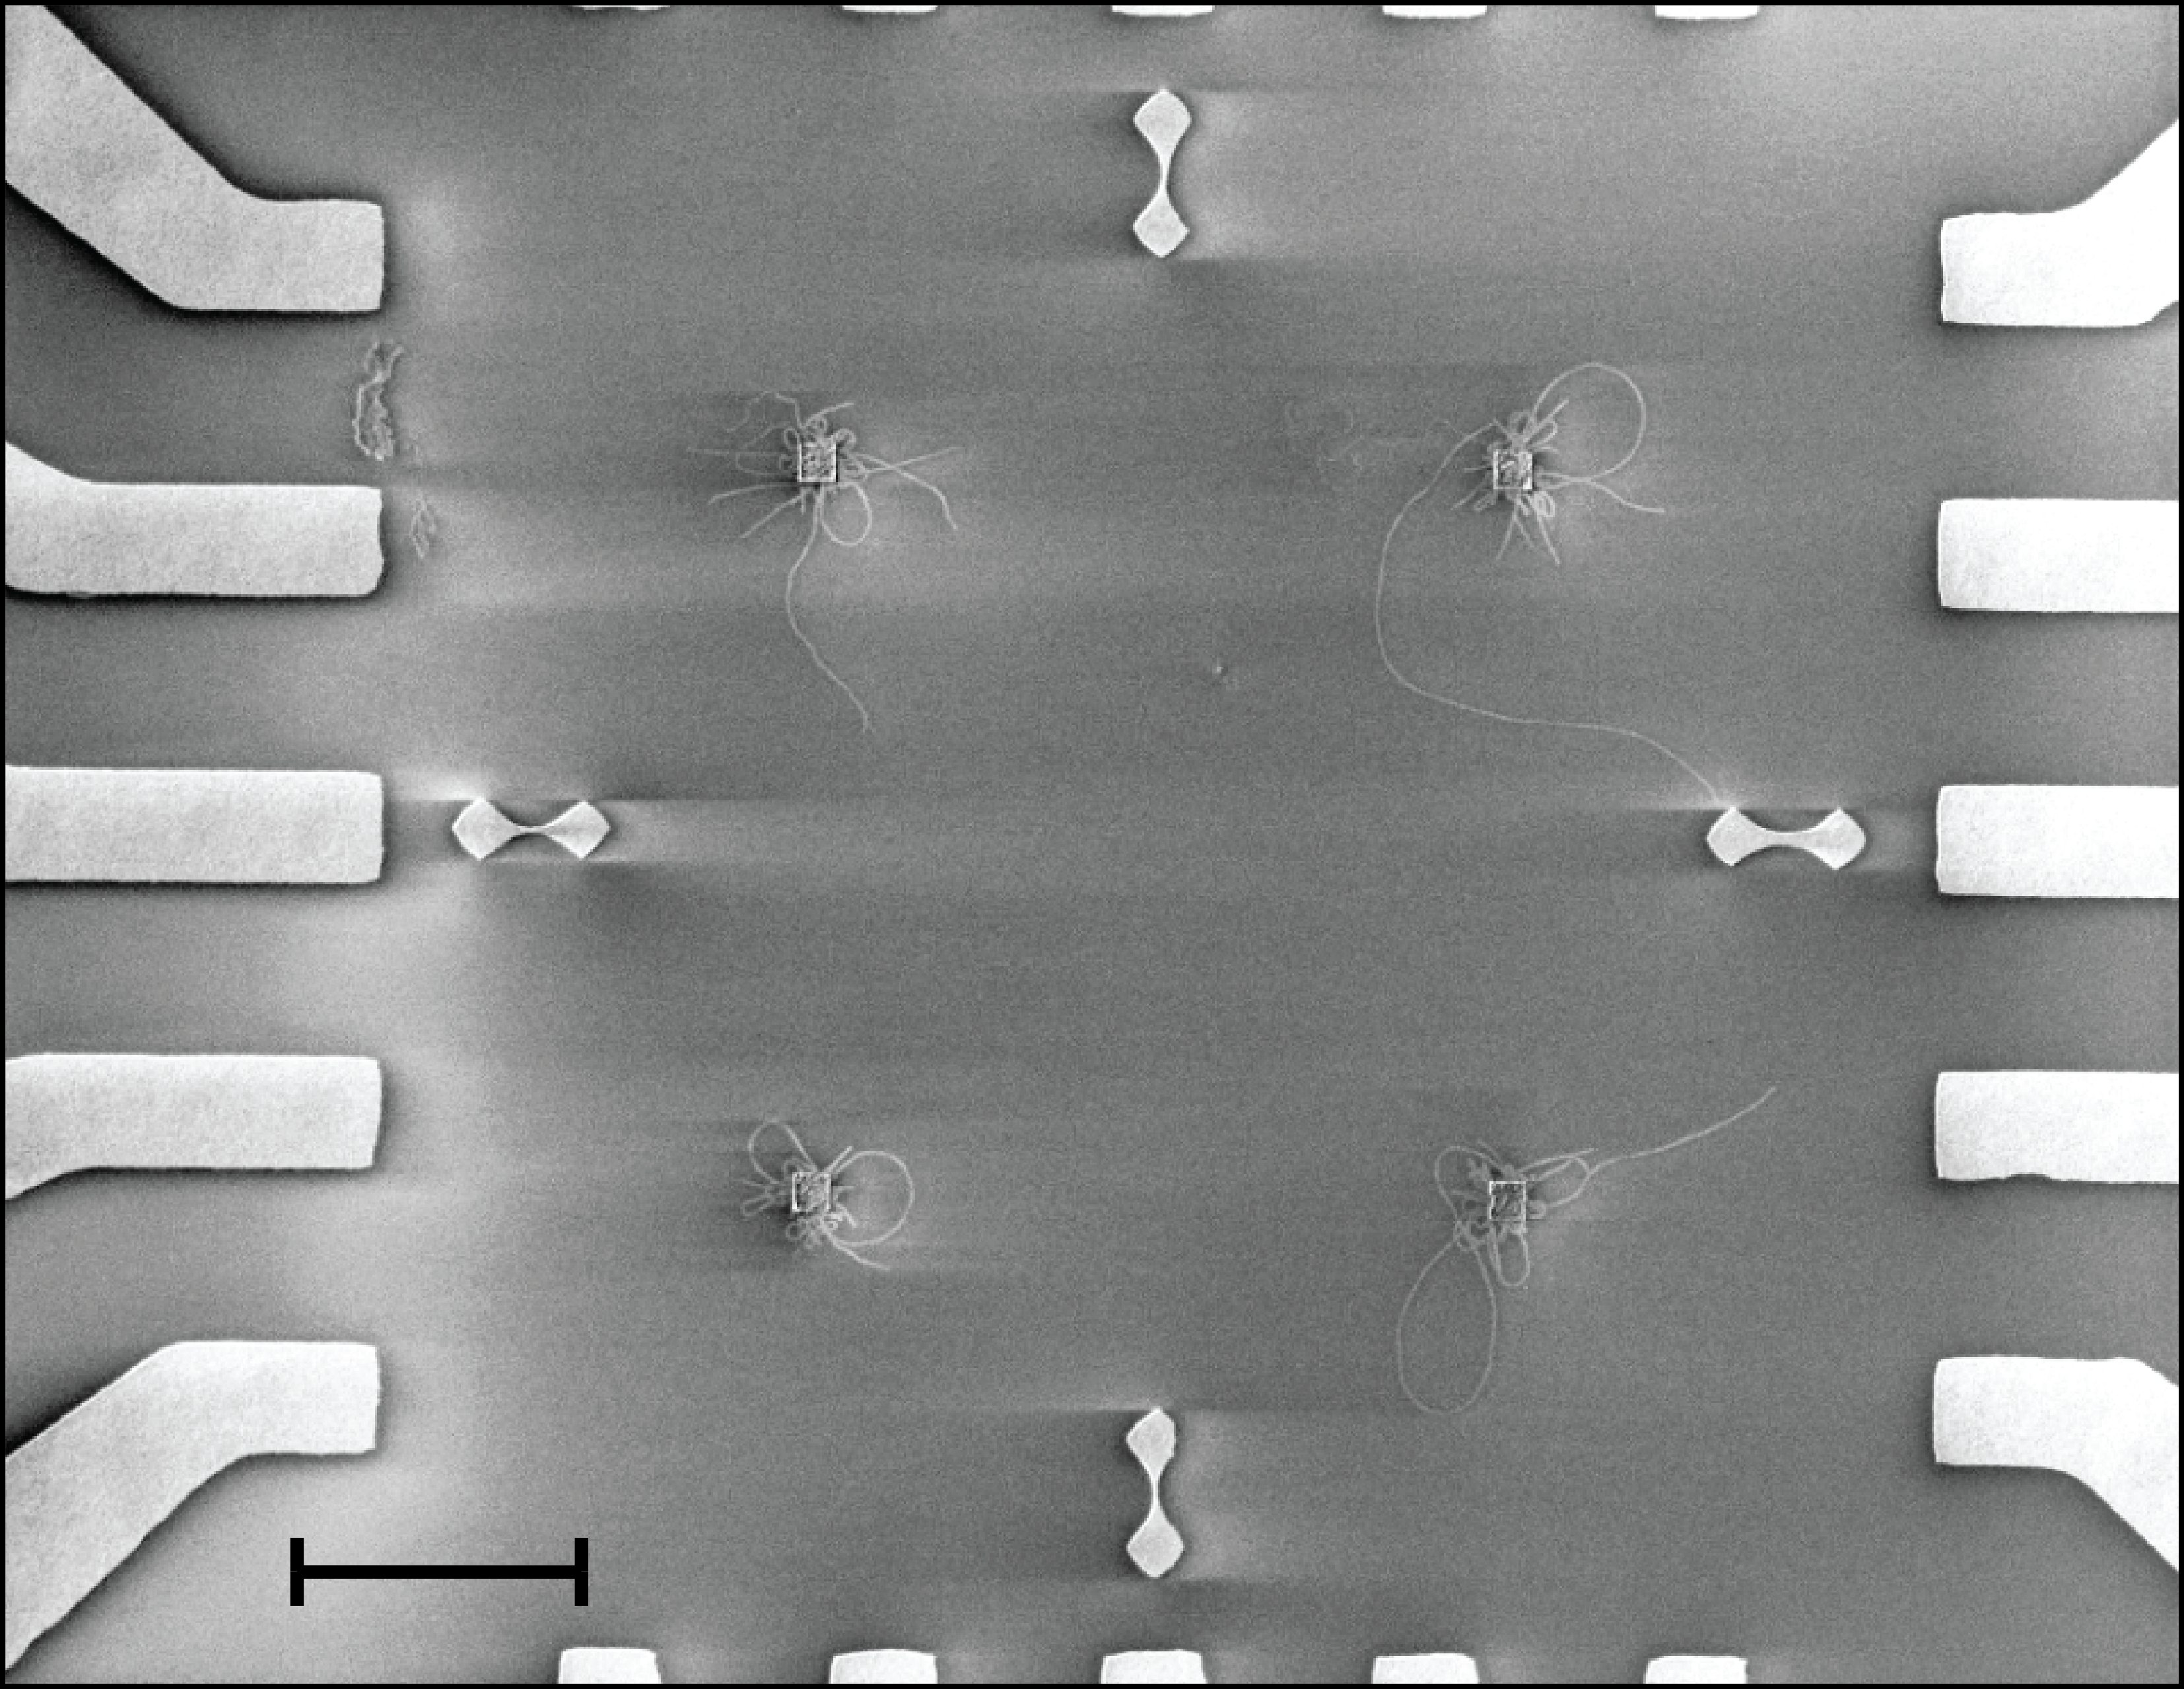
\includegraphics[width = 0.8\textwidth]{chapter3/sem_islands.eps}
	\caption{A scanning electron micrograph of a catalyst island sample after nanotube growth. The scale bar is \SI{10}{\micro\meter}.}
	\label{fig:sem_islands}
\end{figure}

Typically, an EFM scan of a sample will take 45 minutes. A SEM image of the same sample takes less than 2 minutes. However, the SEM can introduce some carbon contamination from the high energy electrons passing through small amounts of oil mist back-streaming into the vacuum chamber from the mechanical roughing pump. Due to the large number of samples that were produced to obtain the data in this thesis, it was decided that contamination from the SEM was an acceptable risk, given the immense time savings.

\section{Image Filtering}

Once it became clear that the scanning electron microscope was by far the most efficient and reliable way to locate carbon nanotubes on a substrate, it also became important to optimize those images to revel the most information possible. The resolution and contrast in the SEM images produced in our lab are limited due the the use of a thermionic \ce{LaB6} filament. Unlike field emission scanning electron microscopes, which are more common in nanofabrication, the thermionic scanning electron microscope has a large initial crossover size, requiring more electromagntic lens focusing to produce a sufficiently small beam size for imaging. This problem is exasperated when using low accelerating potentials (500-\SI{3000}{\volt}), which are crucial to achieving good contrast of carbon nanotubes on a silicon substrate.

\subsection{Histogram Equalization}

This method was based on two corrections. First, a plane fit to correct for the position of the secondary electron detector. Second, finding the histogram of all o

\subsection{Matched Filter Bank}

Matched filter banks are a well known technique that have been used very successfully to filter retinal images in medicine \cite{Chaudhuri1989}. This technique has previously been adapted to high resolution images of SEM bundles \cite{Guerrero2014}. The following section describes the implementation of this method to filter images of single walled carbon nanotubes grown on insulating substrates. 
%% nanotube profiles -> kernel -> filtering/thresholding

\subsubsection{Nanotube Profile Model}

To begin building the matched filter bank, the profile shape of a single nanotube from the SEM image must be determined. To find this shape, a random set of 25 SEM images was selected. From each of these images, two nanotubes were chosen. Those nanobues can be seen in Figure (...)a. Each of these images was then rotate such that the longest, straight portion that could be identified by eye was oriented vertically. The profile of the nanotube was averaged over that long straight section. These results are plotted in ...

% figures I want for this section...
% 1. original data set
% 2. extracted profiles with fits, histograms of k, L data
% 3. filter bank, each filter applied, original image, result

Based on the shape of these profiles a truncated sinc function was chose to fit the nanotube profile. 

%% equation for sinc function including truncated region

This fuction was chosen because it captures the dark regions beside the nanotube, while still only requiring one fit parameter.

\subsubsection{Filter Kernel}

\subsubsection{Results}
\appendix
\chapter{Fabrication Details}
\label{chap:fabrication}
\chaptermark{Fabrication Details}

This appendix describes, in detail, each of the steps taken to create the carbon nanotube (nanotube) devices measured for this thesis. Some of the information is specific to the Markovic lab and Johns Hopkins University, but an effort has been made to make the discussion useful to anyone producing nanotube devices.

The devices measured in this thesis were all produced with the following recipe:

\begin{enumerate}
\item Use the mask aligner (\ref{subsubsec:mask_aligner}) to pattern large sputtered molybdenum (\ref{subsec:sputtering}) leads on a silicon substrate
\item Pattern small catalyst islands (\ref{subsec:catalyst_island}) using electron beam lithography (\ref{sec:ebeam_lith})
\item Grow nanotubes directly on substrate using chemical vapor deposition (\ref{subsubsec:substrate_cvd})
\item Locate nanotubes using a scanning electron microscope (\ref{subsubsec:imaging_island})
\item Design devices using vector graphics software (\ref{sec:device_design})
\item Pattern devices using electron beam lithography (\ref{sec:ebeam_lith}) and thin film deposition (\ref{sec:thin_film})
\item Test device connectivity in the DC probe station (\ref{subsec:probe_station})
\item Wire bond connected devices in a chip carrier for further testing (\ref{subsec:wire_bonding})
\end{enumerate}

For details on each of the steps see the sections referenced. The rest of this appendix discusses additional methods and contains some useful observations made over several years spent producing nanotube devices.

\section{Wafer Preparation}

Each nanotube device began with a highly doped silicon substrate capped with an insulating layer. The wafers used were chosen for their low temperature electrical properties and ease of use.

\subsection{Selection and Cleaning}

All of the devices discussed in this thesis were built on highly n-doped silicon wafers with \ce{SiO2} capping layers. The wafers were purchased from Silicon Quest International. As ordered the wafers are 3 inches in diameter with a <100> silicon face. This crystal alignment allowed the wafers to be easily cleaved along the crystal axes using only a diamond scribe. The wafers are heavily n-doped with phosphorus giving them a resistivity of 10-\SI{20}{\ohm\centi\meter} down to the milliKelvin range. The oxide layers were \SI{300}{\angstrom} of thermally grown \ce{SiO2} and remained insulating at all measured temperatures.

Typically, wafers were cleaned by sonicating in acetone for 5 minutes, followed by an isopropanol rinse for 1 minute, and baking on a hot plate at about \SI{180}{\degreeCelsius} for 1 minute. This procedure was usually enough to ready the surface for lithography. In cases where cleanliness had to be improved, piranha etch was used to clean the wafers. 

Pirana etch is a mixture of 3:1 30\% sulfuric acid to 30\% hydrogen peroxide. It is important to be extremely careful with this wet etch as the solution is strongly exothermic. The wafers should be placed in the sulfuric acid, then the hydrogen peroxide is added slowly while stirring continuously. The solution will reach nearly \SI{200}{\degreeCelsius} within the first few minutes. After about 20 minutes, the solution should cool enough for the wafers to be removed. Surfaces cleaned in this way are free of organic and most metallic contaminates.

\subsection{Optical Lithography}
\label{subsec:optical}

The first step in building the devices discussed in this thesis was to pattern the substrate using optical lithography. In this process the wafer is first coated in a UV sensitive polymer resist. The wafer is then partially exposed to UV light and developed, leaving a patterned polymer mask through which thin films can be deposited.

The resists used can be either positive or negative tone. For this work, MicroChem S1813 was used as a positive tone resist and Futurex NR9 was the negative tone resist. Exposure, baking, and development times were chosen according to the manufacturer's instructions.

\subsubsection{Projection Lithography}
\label{subsubsec:project_lith}

Many of the devices produced in the Markovic lab have been patterned using the custom built projection lithography setup seen in Figure \ref{fig:project_lith}. The setup was built around a Nikon optical microscope. The microscope has been fitted with a UV lamp, movable UV filtering, and a custom mask holder.

\begin{figure}
    \centering
    \includegraphics[width = 1.0\textwidth]{appa/project_lith.eps}
    \caption{Custom projection lithography setup in the JHU physics department cleanroom. (a) The arrows from left to right show the UV lamp, sliding UV filter, and mask holder. (b) A projection lithography mask and holder. The arrow shows the mask itself.}
    \label{fig:project_lith}
\end{figure}

The masks were made using either a standard ink-jet printer or by a local printing company for higher resolution. The sample is placed under the desired objective, which determines the size of the pattern projected onto the sample. The mask is then inserted into the holder and then focused and positioned using the micrometer drives. Exposure times are  controlled by removing the UV filter from the light path. 

This setup is useful for quickly producing a few samples at a time. Specifically, it is used for producing graphene and nanowire devices, which require careful positioning of the pattern over the nanostructure of interest. The resolution limit of this technique is about \SI{2}{\micro\meter}. 

\subsubsection{Mask Aligner}
\label{subsubsec:mask_aligner}

For production of many, identical devices, projection lithography as described in Section \ref{subsubsec:project_lith} becomes extremely tedious. This problem was solved by use of a mask aligner. 

\begin{figure}
    \centering
    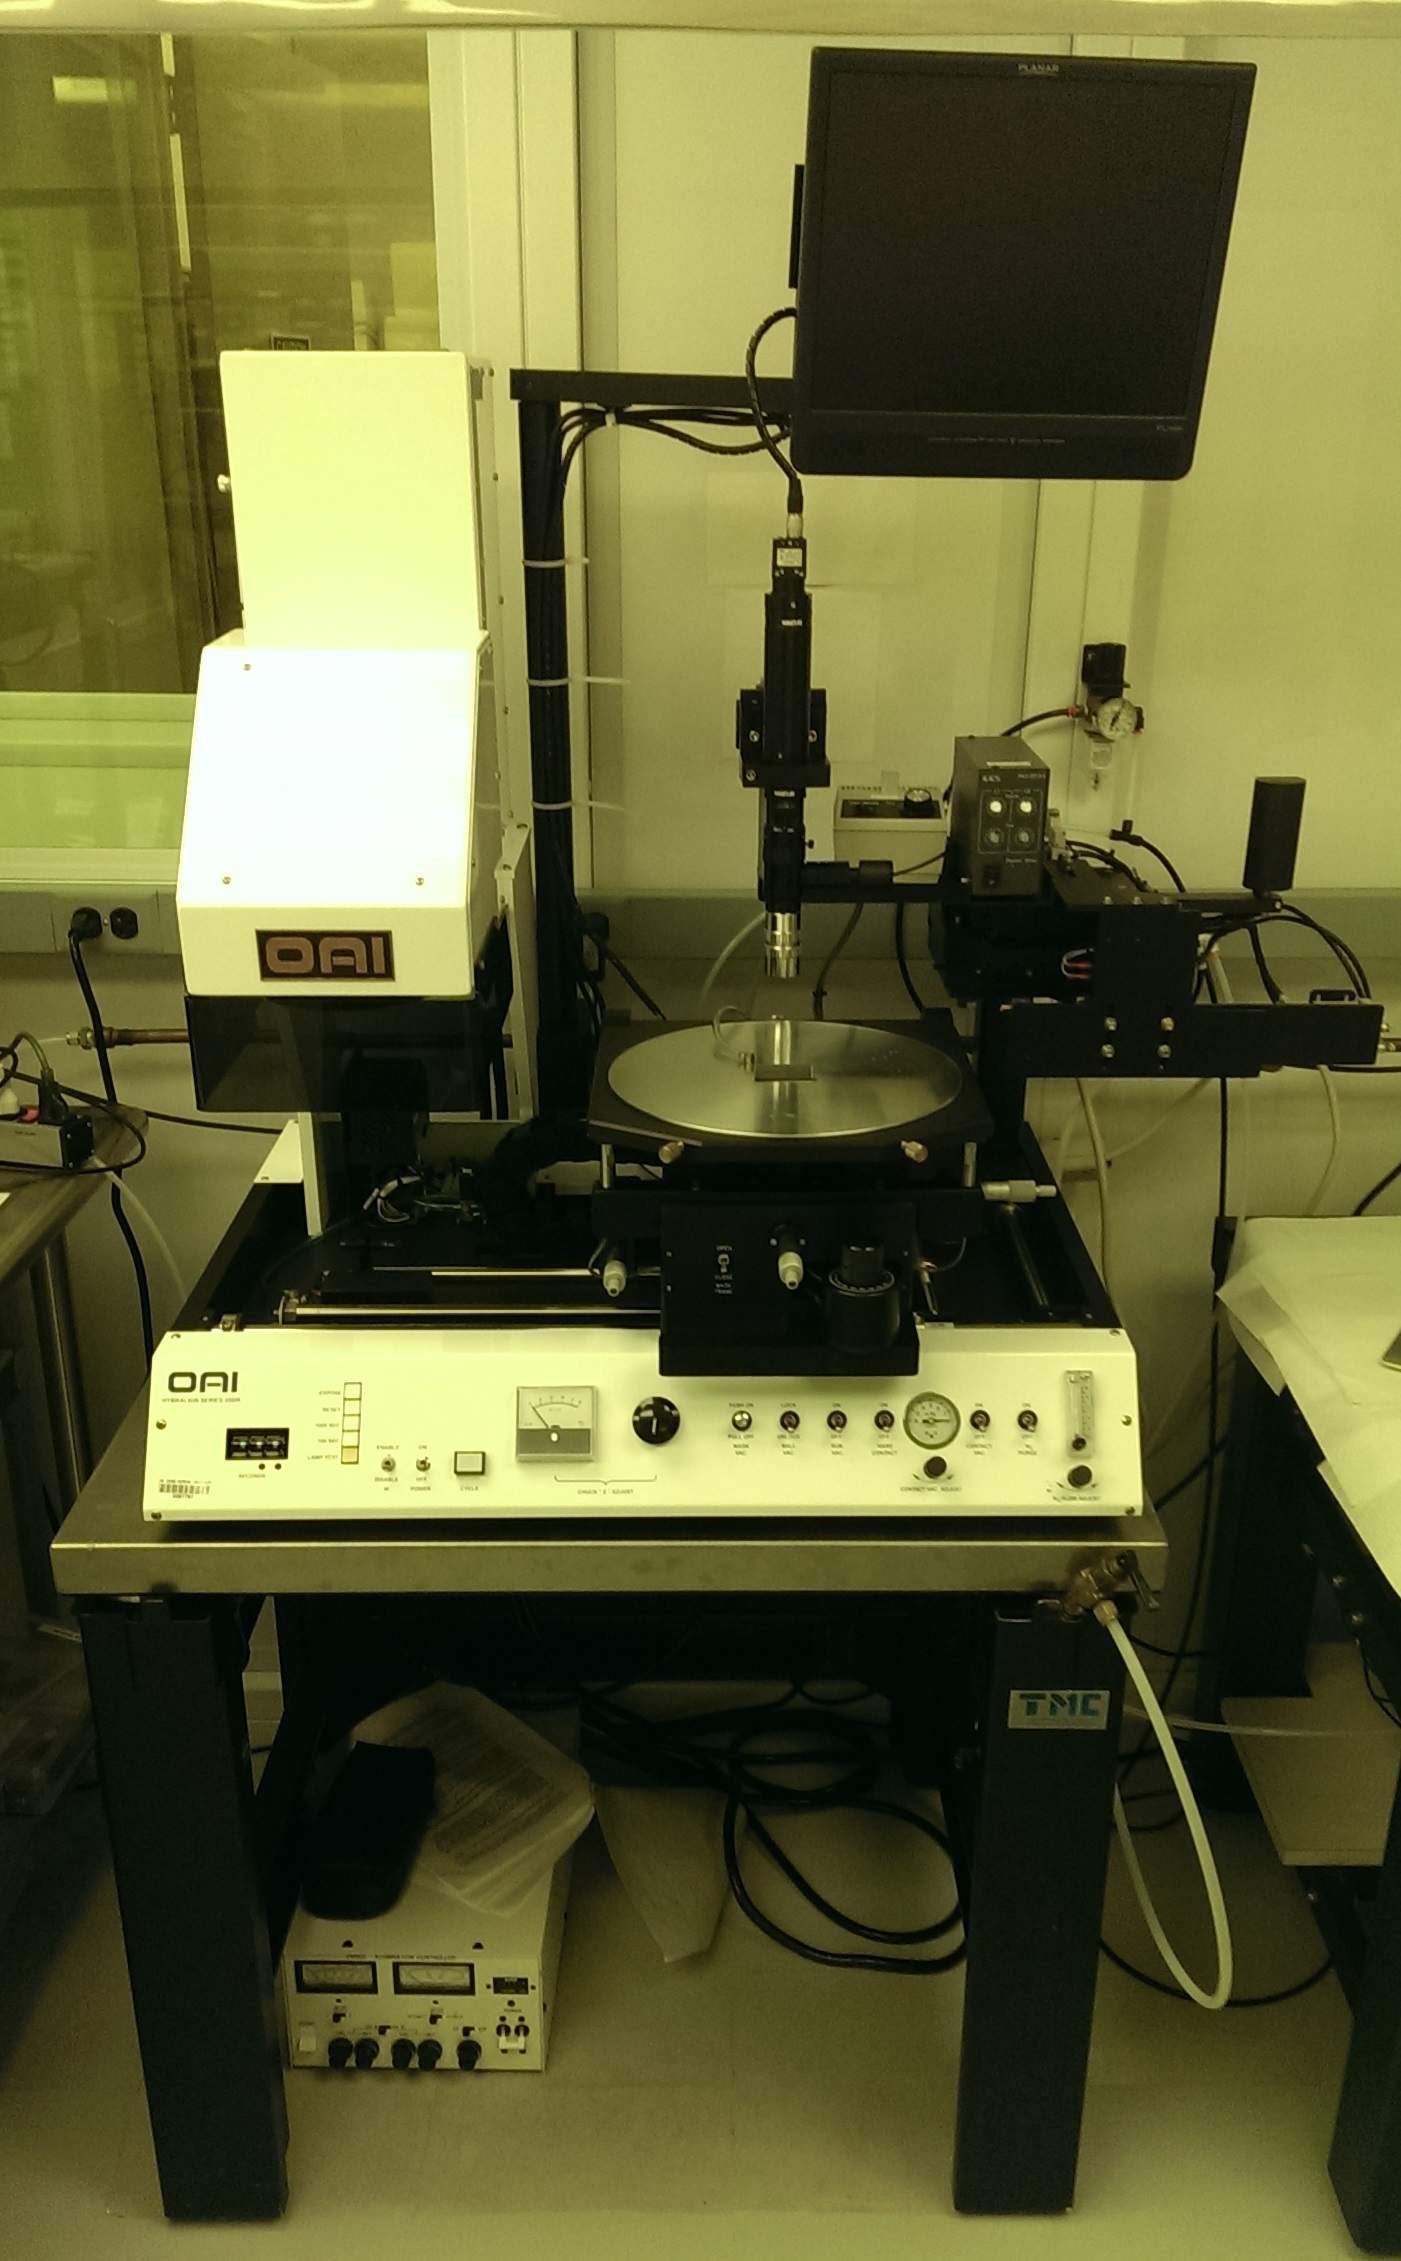
\includegraphics[width = 1.0\textwidth]{appa/mask_aligner.eps}
    \caption{OAI mask aligner in the JHU physics department cleanroom. (a) The mask aligner. (b) A typical 3" chromium on glass mask.}
    \label{fig:mask_aligner}
\end{figure}

First, a chromium on glass mask is made with the desired pattern in the actual size, as seen in Figure \ref{fig:mask_aligner}. The mask is then loaded into the aligner and a substrate, coated with polymer resist, is mounted under it. Finally, the mask and substrate are pressed together and exposed to a UV light source. The resolution of the OAI mask aligner is about \SI{1}{\micro\meter}.

\section{Device Design}
\label{sec:device_design}

Once the substrates are prepared, devices are designed one at a time using Adobe Illustrator. Any computer aided drafting (CAD) or vector graphics program would work just as well. The procedure is outlined in Figure \ref{fig:device_design}. Designing the devices is a simple process of connecting the nanotubes with the mask aligner leads, although some thought must be given to the size of the leads drawn. If the leads are too large, the write time for the electron beam lithography steps will be too long. Additionally, one must be careful not to let any stray nanotubes short the device leads.

\begin{figure}
	\centering
	\includegraphics[width = 1.0\textwidth]{appa/device_design.eps}
	\caption{Adobe Illustrator designs used for optical and electron beam lithography masks. (a) The pink outlines show the large molybdenum leads patterned with the mask aligner. Inside that pattern are the four \SI{3}{\micro\meter} catalyst islands patterned with electron beam lithography. (b) An SEM micrograph of a sample after CVD growth fitted into the pattern. (c) A complete circuit design. In this case, the layers are normal metal (green), ferromagnet (purple), and superconductor (blue).} 
	\label{fig:device_design}
\end{figure}

\section{Electron Beam Lithography}
\label{sec:ebeam_lith}

Electron beam lithography is the process of creating masks by patterning a polymer resist by exposure to a focused beam of electrons. In the Johns Hopkins physics department the electron beam lithography setup is based around a Zeiss EVO50 scanning electron microscope. The microscope is controlled by Zeiss SmartSEM software. Attached to the microscope control computer by a serial port is a second computer running Elphy Quantum, electron beam lithography software from Raith. The Raith software can take control of the beam to write patterns based on GDSII drawings. The SEM setup is shown in Figure \ref{fig:sem_setup}.

\begin{figure}
	\centering
	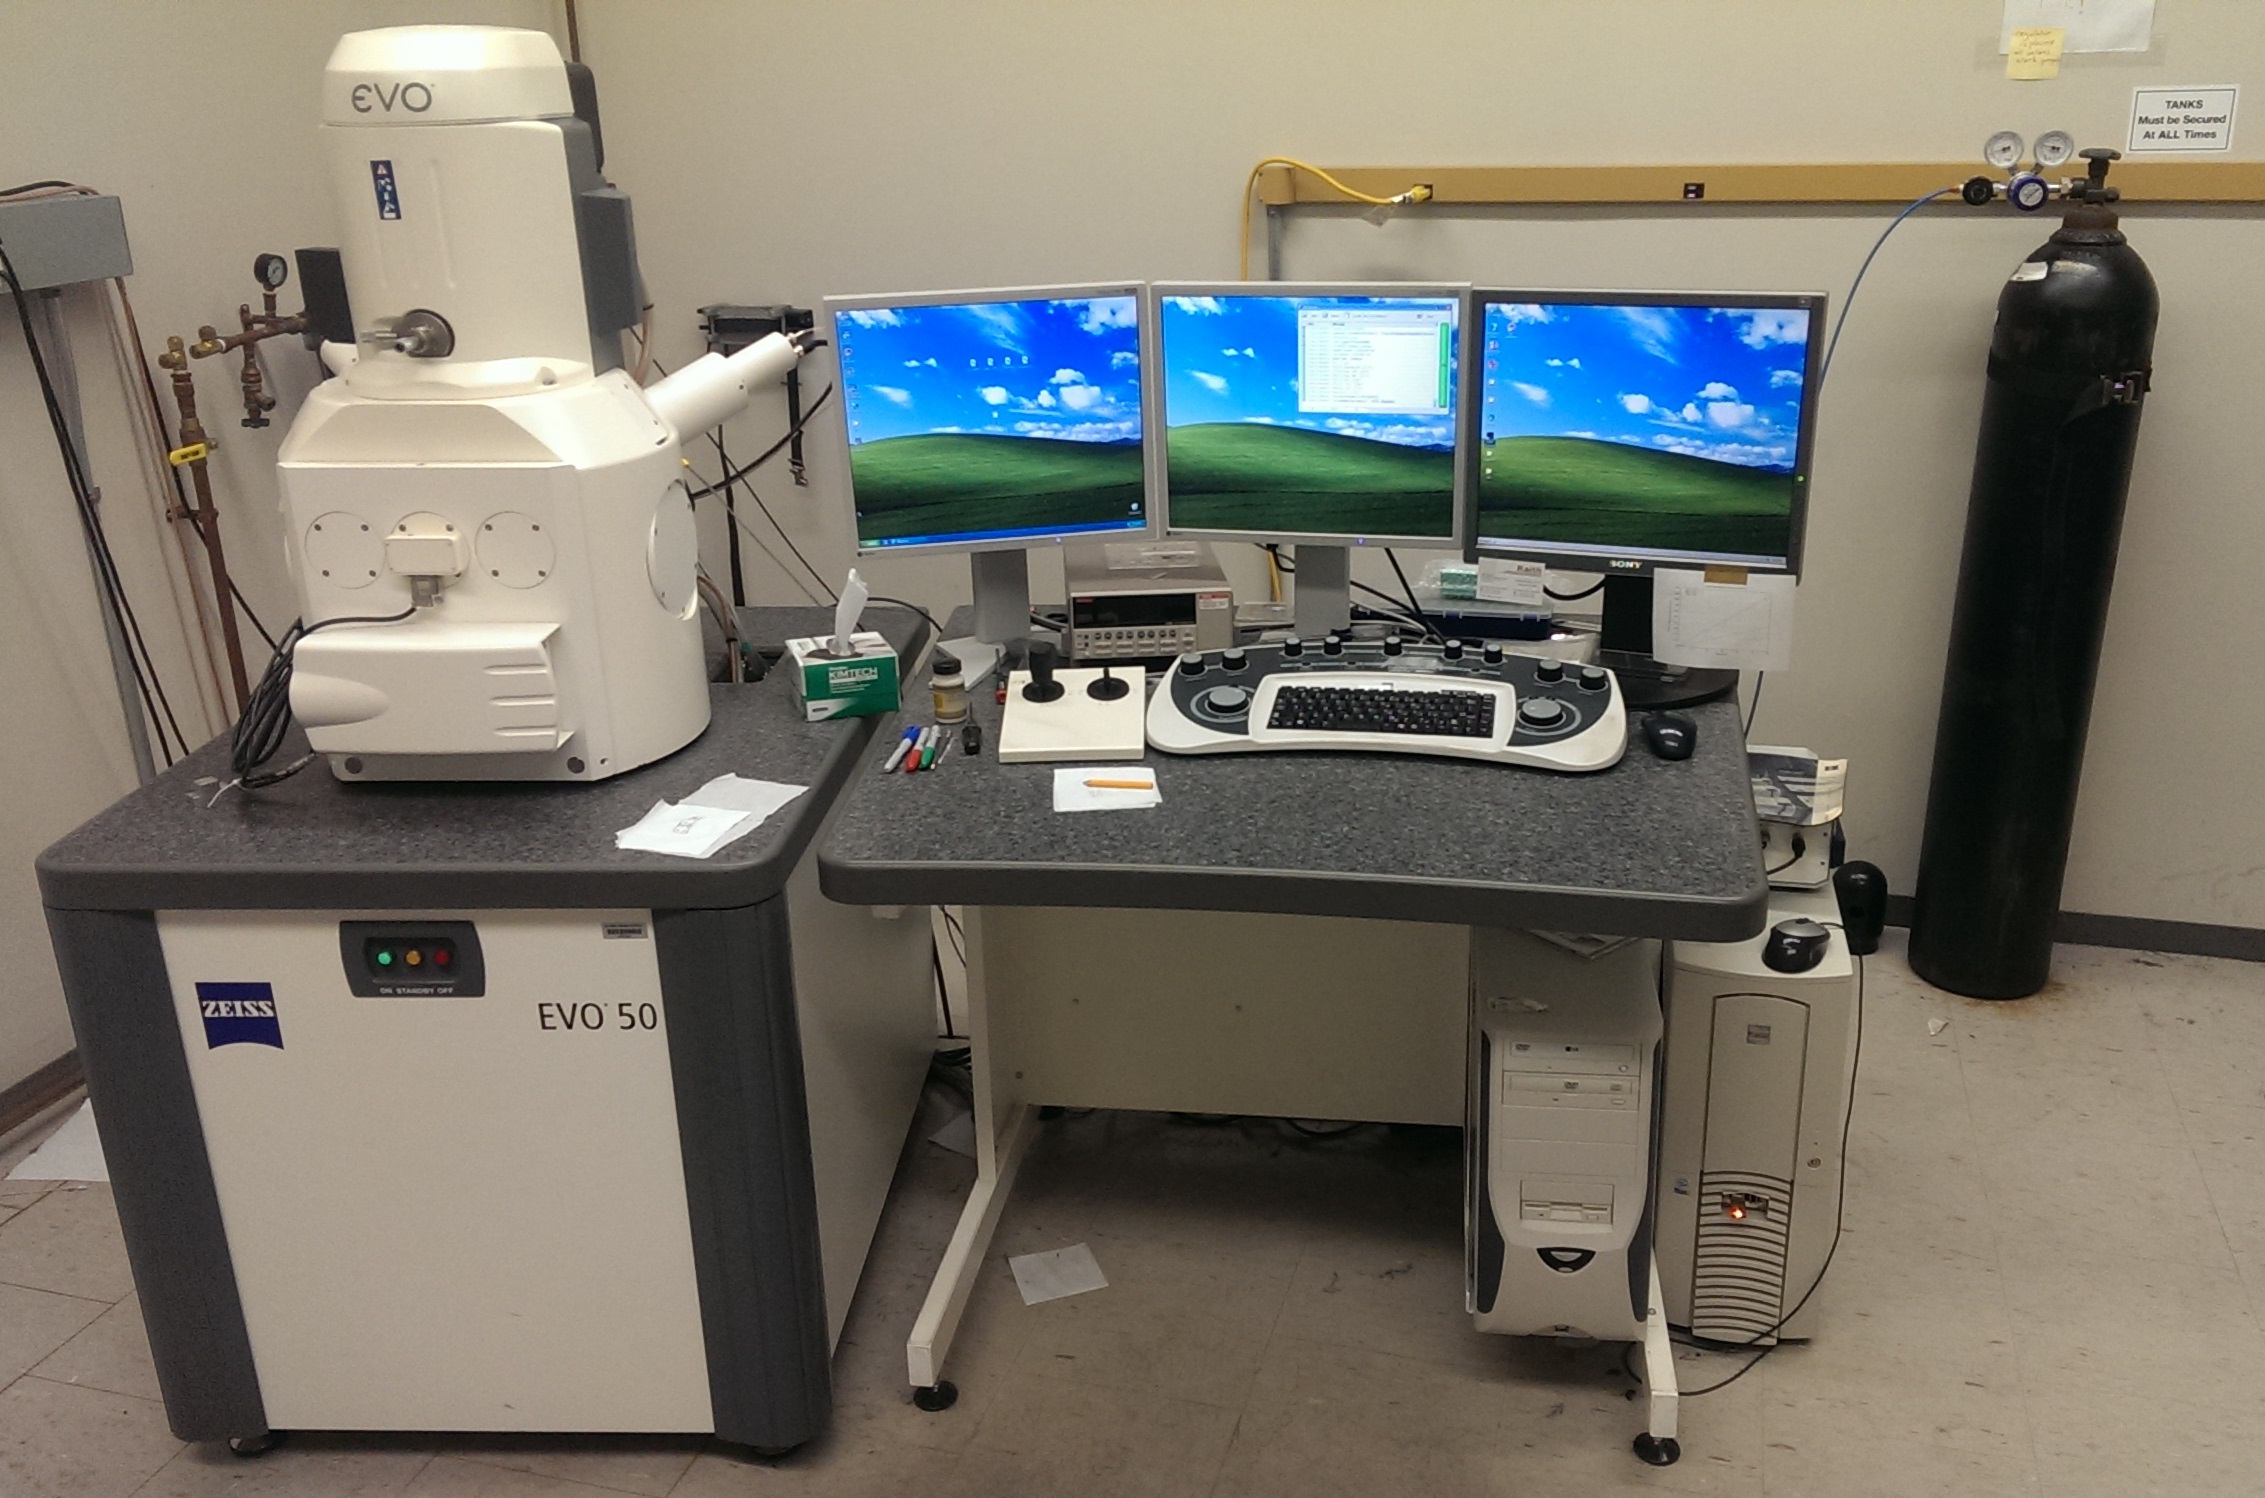
\includegraphics[width = 0.8\textwidth]{appa/sem_setup.jpg}
	\caption{Zeiss EVO50 SEM with Raith control computer and external beam blanker.}
	\label{fig:sem_setup}
\end{figure}

The electron beam sensitive resist used in all of this work was polymethyl methacrylate (PMMA) from MicroChem. PMMA is a polymer that, after baking on a hot plate, forms copolymer bonds that can be broken by exposure to a beam of electrons. Once these bonds are broken, the unbonded polymer can be washed away by a developer, leaving trenches in the PMMA wherever it was exposed to the electron beam. The patterned mask can later be removed by soaking in acetone.

\subsection{Standard Recipe}

\begin{table}
	\centering
	\caption{Standard PMMA/MIBK recipe}
	%\hfill \\
    \begin{tabular}{ r | l }
    	\hline
    	EHT Voltage & \SI{30}{\kilo\electronvolt} \\ \hline
    	Beam Current & \SI{40}{\pico\ampere} \\ \hline
    	Step Size & \SI{10}{\nano\meter} \\ \hline
    	Dose & \SI{300}{\micro\coulomb\per\square\centi\meter} \\ \hline
    	Developer & 1:3 MIBK:IPA \\ \hline
    	Development time & 60s \\ \hline
    	Post-development & rinse 30s in IPA \\ \hline
    \end{tabular}
    \label{table:standard_pmma}
\end{table}

This recipe, using room temperature methyl isobutyl ketone (MIBK) as a PMMA developer, is the simplest recipe to start with for almost any project requiring electron beam lithography. The relevant parameters are shown in Table \ref{table:standard_pmma}.

\subsection{Cold Development}

\begin{table}
	\centering
	\caption{Cold developer recipe}
	%\hfill \\
    \begin{tabular}{ r | l }
    	\hline
    	EHT Voltage & \SI{30}{\kilo\electronvolt} \\ \hline
    	Beam Current & \SI{40}{\pico\ampere} \\ \hline
    	Step Size & \SI{10}{\nano\meter} \\ \hline
    	Dose & \SI{1400}{\micro\coulomb\per\square\centi\meter} \\ \hline
    	Developer & 7:3 IPA:water at \SI{0}{\degreeCelsius} \\ \hline
    	Development time & 90s \\ \hline
    	Post-development & rinse 30s in water \\ \hline
    \end{tabular}
    \label{table:cold_pmma}
\end{table}

It was discovered in 2004, that by lowering the development temperature and increasing the dose, the resolution of PMMA could be improved significantly \cite{Hu2004}. This has been shown using MIBK:IPA as a developer as well as various mixtures of IPA and water \cite{Cord2007, Yasin2002, Rooks2002, Koshelev2011}. The best results obtained in our lab were using IPA and water. The recipe is shown in Table \ref{table:cold_pmma}. The improved contrast can be attributed to the higher dose. By increasing the dose and decreasing the efficacy of the developer, the negative effects of backscattered electrons passing through the PMMA are diminished.

\section{Thin Film Deposition}
\label{sec:thin_film}

In this work, thin film deposition is used (along with polymer masks patterned with optical or electron beam lithography) to create circuits around carbon nanotubes. There are three main methods used; each method will be discussed along with a few materials typically deposited in that way. 

\subsection{Thermal Evaporation}
\label{subsec:thermal_evap}

Thermal evaporation is the simplest method of thin film deposition discussed here. The material to be evaporated is placed in a boat, typically made of tungsten, alumina, or both. Substrates for the film to be deposited on are located above the evaporation boat. Both the boat and the samples are placed in a high vacuum chamber. Once the chamber has reached around \SI{1d-7}{\torr}, current through the evaporation boat is increased until the material melts or begins to sublimate. The deposited thickness and deposition rate are monitored using a quartz crystal monitor. Once the desired rate is reached, a shutter is opened to expose the sample to the evaporated material. 

This type of evaporation is best used with materials that have a relatively low melting point ($\lesssim$\SI{1200}{\degreeCelsius}). Two evaporators were used in this work, a 1970s Denton evaporator fitted with a newer Hewlett Packard power supply, and an early 2000s Torr thermal evaporator. The Torr chamber is kept free from magnetic materials in hopes of limiting contamination of superconducting films. Some common materials and the boats we have found most useful are listed in Table \ref{table:thermal_evap}.

\begin{table}
	\centering
	\caption{Thermal evaporation materials}
	%\hfill \\
	\begin{tabular}{r | p{60mm}}
		\hline
		Au & alumina coated W crucible \\ \hline
		Ti & long, narrow W boat \\ \hline
		Cr & chrome plated W rod\\ \hline
		Al & dimpled W boat \\ \hline
		Co & alumina coated W crucible (does not last long) \\ \hline
	\end{tabular}
	\label{table:thermal_evap}
\end{table}	

\subsection{Electron Beam Evaporation}
\label{subsec:ebeam_evap}

Electron beam evaporation uses a high energy (\SI{7.5}{\kilo\electronvolt}) beam of electrons to melt the source material. The electron gun sits under a crucible full of the source material. The electron beam generated is bent and rastered across the center of the crucible using a strong magnetic field. Substrates are placed above the crucible and as the material melts and evaporates it is deposited on the substrate.

This method of evaporation has two benefits over thermal evaporation. First, it can be used for materials with a higher melting point. In the case of the Sharon Vacuum electron beam evaporator used in this work, materials with melting points up to $\sim$\SI{1800}{\degreeCelsius} were successfully evaporated. Second, the evaporated films are typically a little cleaner because the crucible, unlike thermal evaporation boats, does not have to be heated in order for the source material to melt. 

Due to limited access to the evaporator, not many of the films discussed in this work were deposited with electron beam evaporation. However, we have successfully deposited Nb, Co, Ti, and Al films all from graphite crucibles. Graphite was chosen here because of its affordability. There are likely better choices of crucible available. 

\subsection{Sputtering}
\label{subsec:sputtering}

Magnetron sputtering is a great method to deposit an amorphous thin film of just about any material needed. The three-target sputtering chamber used in this work was custom built by Professor Chia-Ling Chien's group at Johns Hopkins.

To sputter a material, a target 1-2 inches in diameter is loaded onto a cathode at the bottom of a vacuum chamber. The substrate to be coated is placed above the target on the anode. Once the system is at high vacuum,  argon gas (or any inert gas) is introduced to the chamber. An argon plasma is ignited between the cathode (target) and anode (sample). The strong electric potential and magnetic field from permanent magnets placed under the target focus the plasma in a ring pattern on the face of the target. Argon ions bombard the target and target atoms are ejected toward the substrate mounted above. 

The benefit of sputtering, as mentioned above, is that almost any metal can be sputtered with a DC plasma (RF plasma is used for insulating materials). Due to the high energy of the argon ions and ejected target atoms, this method can damage some sensitive samples. There may be some evidence that this is the case with carbon nanotube samples. For this work, low energy plasma was used to keep the average energy of ejected target atoms around a few eV. This is about 10 times higher than the energies used in thermal and electron beam evaporation. Even if sputtering does introduce some damage to nanotube samples, it does not appear to be the primary source of disorder.

\subsection{Atomic Layer Deposition}
\label{subsec:ald}

\begin{figure}
	\centering
	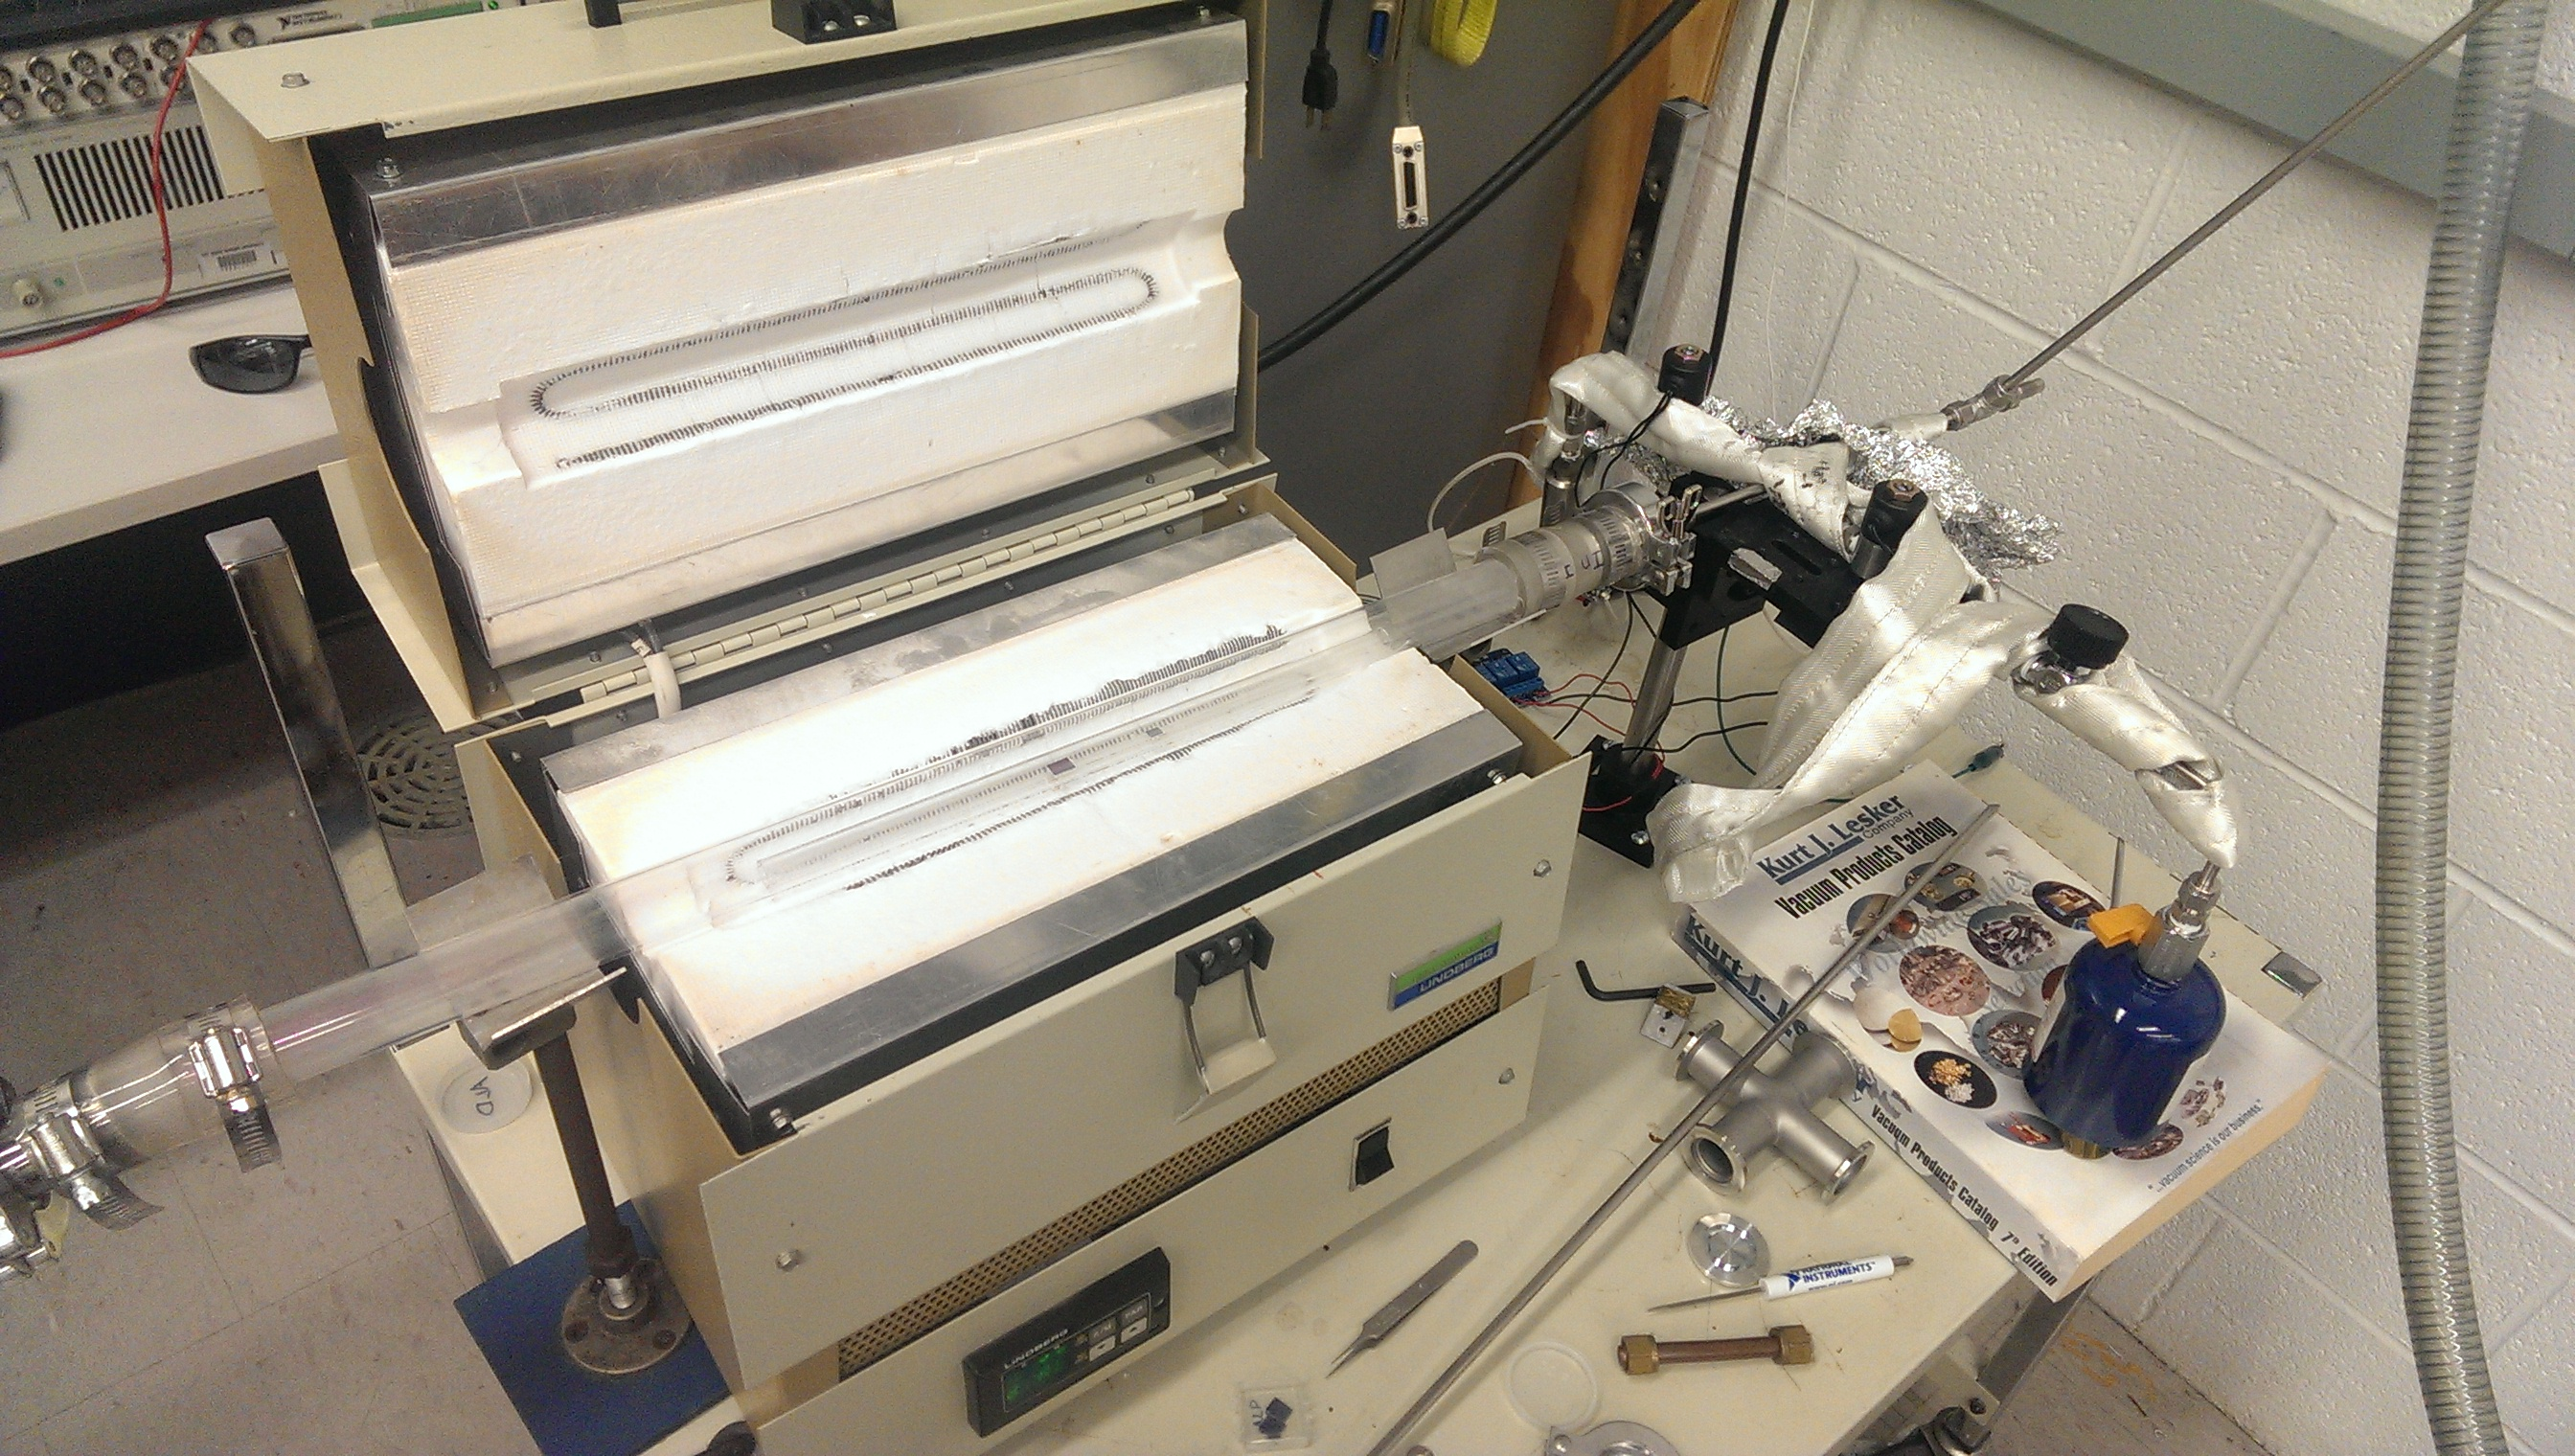
\includegraphics[width = 0.8\textwidth]{appa/ald.jpg}
	\caption{The Markovic lab ALD reactor. Gas flow is from right to left.} 
	\label{fig:ald}
\end{figure}

Atomic layer deposition (ALD) is a process in which thin, usually insulating, films are grown by reacting a series of gases. As a part of this work, we have constructed a homemade ALD reactor in the Markovic lab with the help of Streit Cunningham. It uses the same Lindberg 1 inch tube furnace as the chemical vapor deposition setup.

Samples are loaded into a 1 inch quartz tube and placed in the furnace. The tube is evacuated to about \SI{100}{\milli\torr} using a mechanical rough pump. A high purity \ce{N2} flow is turned on and adjusted so the pressure in the chamber, with the pump still running, is \SI{1000}{\milli\torr}. The \ce{N2} flow will act as a carrier gas throughout the process. We have only tested the reactor for growth of \ce{Al2O3} layers. Two precursor gases are used in the growth of \ce{Al2O3}, water vapor and trimethylaluminum (TMA). Once the quartz tube is evacuated and \ce{N2} flow is set, the water vapor and TMA are alternately pulsed using computer controlled solenoid valves. Films grow one monolayer (\SI{1.1}{\angstrom}) per pulse cycle. A typical recipe is as follows:

\begin{enumerate}
\item Evacuate tube to \SI{100}{\milli\torr} with mechanical pump
\item Turn on \ce{N2} flow such that the pressure reaches \SI{1000}{\milli\torr}
\item Set furnace temperature to \SI{130}{\degreeCelsius}
\item Pulse TMA for 1 second
\item Purge for 60 seconds
\item Pulse water for 1 second
\item Purge for 60 seconds
\item Repeat pulse\slash purge cycle until desired thickness has been reached
\item Cool furnace, turn off \ce{N2} flow, turn off pump, remove sample
\end{enumerate}

The goal with this recipe is to grow a quality insulating layer at a temperature low enough to be compatible with PMMA processing. This design is based on previous low temperature ALD growth by the George lab at the University of Colorado Boulder \cite{Elam2002, Groner2004}.

\subsection{Liftoff}
\label{subsec:liftoff}

When patterning a thin film using a polymer mask, such as PMMA or S1813, the final step after deposition of the film is to remove the mask. This process is called liftoff, as the excess metal is lifted off the substrate along with the dissolved polymer mask.

Typically, liftoff is very simple. The sample is soaked in acetone for 1-12 hours (depending on what else is going on in the lab), then rinsed in IPA for 30 seconds followed by a 30 second rinse in water. 

To help remove any stubborn material the sample can be sprayed with a bottle of acetone for a few seconds before rinsing in IPA. Some samples can also be placed in a beaker of acetone in a sonicator for a few seconds before rinsing in IPA. Sonication is not ideal for nanotube samples, as the process tends to break nanotubes off of the substrate and introduce defects in long tubes. An example of this can be seen in Figure \ref{fig:broken_tube}.

\begin{figure}
	\centering
	\includegraphics[width = 1.0\textwidth]{appa/broken_tube.eps}
	\caption{(a) A substrate with catalyst islands and a few long nanotubes before patterning. (b) The same substrate after patterning and liftoff. Comparing the two images, it is clear that the use of sonication during liftoff has broken many of the nanotubes.}
	\label{fig:broken_tube}
\end{figure}

\section{Room Temperature Testing}

After devices have been fabricated, it is important to check the connectivity of the devices before spending the time to load samples into a cryostat.

\subsection{Probe Station}
\label{subsec:probe_station}

The first step after fabrication is to test the resistance, and sometimes the gate behavior, of a device using a DC probe station. Our DC probe station was custom built for our lab and can be seen in Figure \ref{fig:probe_station}.

\begin{figure}
	\centering
	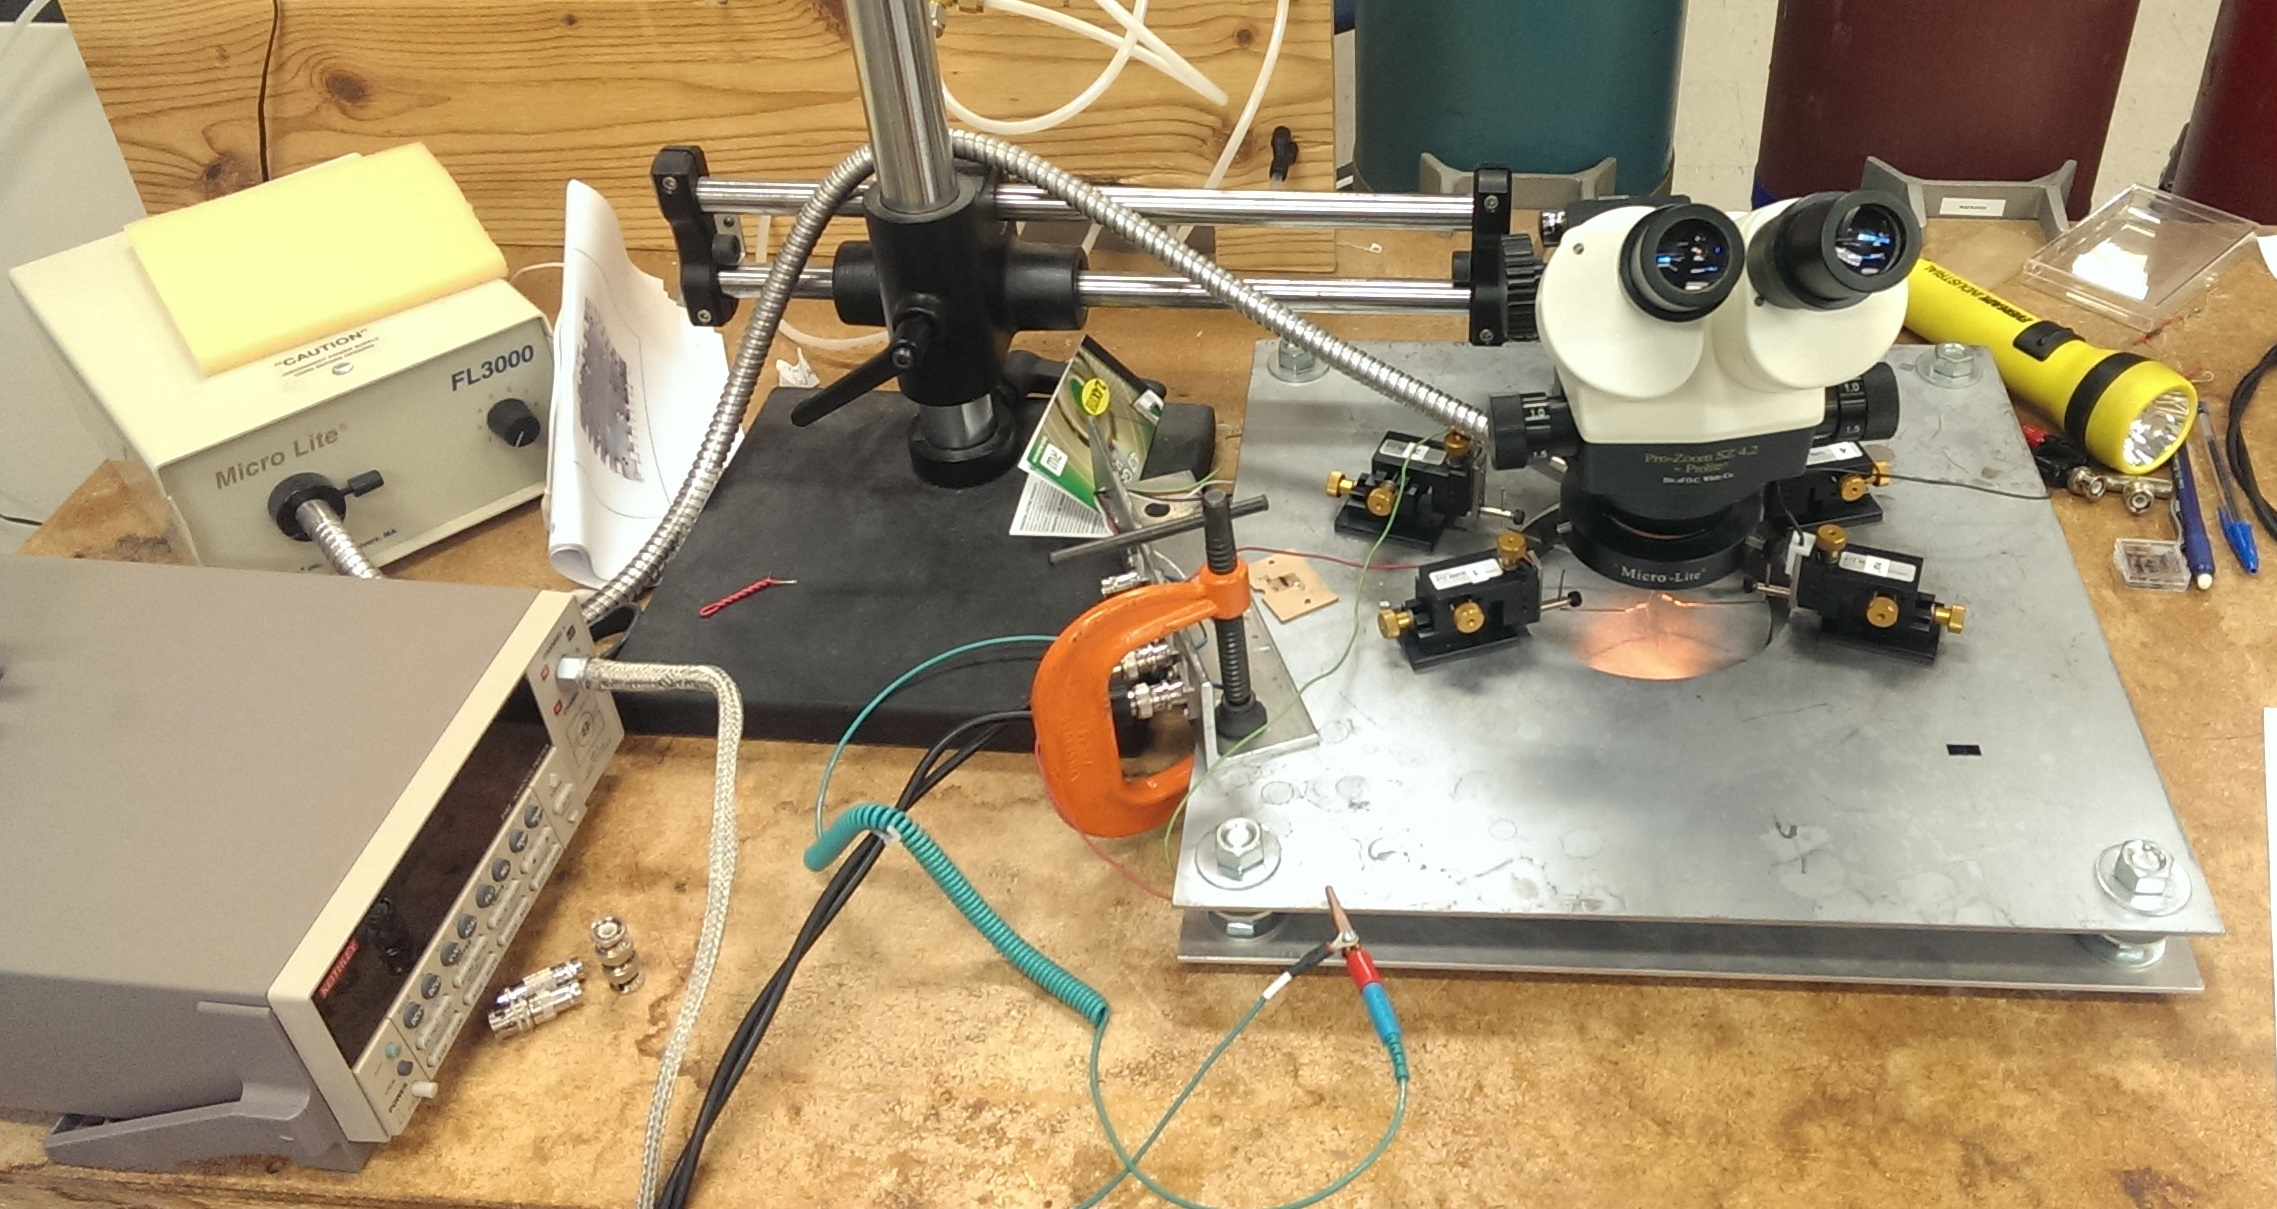
\includegraphics[width=0.8\textwidth]{appa/probe_station.jpg}
	\caption{The Markovic lab probe station. Four sharp probes are located under an optical microscope. Each can be connected to external sources and measurements using BNC connectors.}
	\label{fig:probe_station}
\end{figure}

The simplest and safest way found to check nanotube devices is to apply a small DC voltage (a few \si{\milli\volt}) between two of the large leads and measure the current with an ammeter. The measurements are done using a real-time LabView program. The bias is supplied by a National Instruments DAQ board through a $10^{-2}$ voltage divider. Current is measured by the same DAQ board by monitoring the output of an Ithaco 1211 current-to-voltage amplifier. 

\subsection{Wire Bonding}
\label{subsec:wire_bonding}

The final step in preparing devices for measurement is to wire bond the sample into a chip carrier. Each chip carrier is about \SI{1}{\centi\meter} square and fits into a standard socket on each of our cryostats. The wire bonder is used to connect the large optical lithography leads on the sample to the chip carrier. An old Kulicke and Soffa wire bonder in Chia-Ling Chien's lab was used for this work. It can be seen in Figure \ref{fig:wire_bonder}a.

\begin{figure}
	\centering
	\includegraphics[width=1.0\textwidth]{appa/wire_bonder.eps}
	\caption{(a) Kulicke and Soffa wire bonder. (b) An optical image of a completed device mounted in a chip carrier. (c) An SEM image detailing aluminum wires bonded to large gold leads.}
	\label{fig:wire_bonder}
\end{figure}

The wire bonder is used to connect a point on the chip carrier to a point on the sample with an aluminum or gold thread. The thread is first pressed by the wire bonder tip onto a bonding pad on the chip carrier. When the wire is in contact with the bonding pad the tip vibrates and presses down onto the sample to fix the wire into place. The tip can then be moved to contact one of the large optical lithography leads on the sample with the same wire. Once the second bond is made, the tip pulls away quickly to break the wire. The results of this process can be seen in Figures \ref{fig:wire_bonder}b and c.

%\include{appendixb}

%% REFERENCES

% if you use BIBTEX
\bibliographystyle{IEEEtran}
\bibliography{thesis}

\begin{vita}

%\begin{wrapfigure}{l}{0pt}
%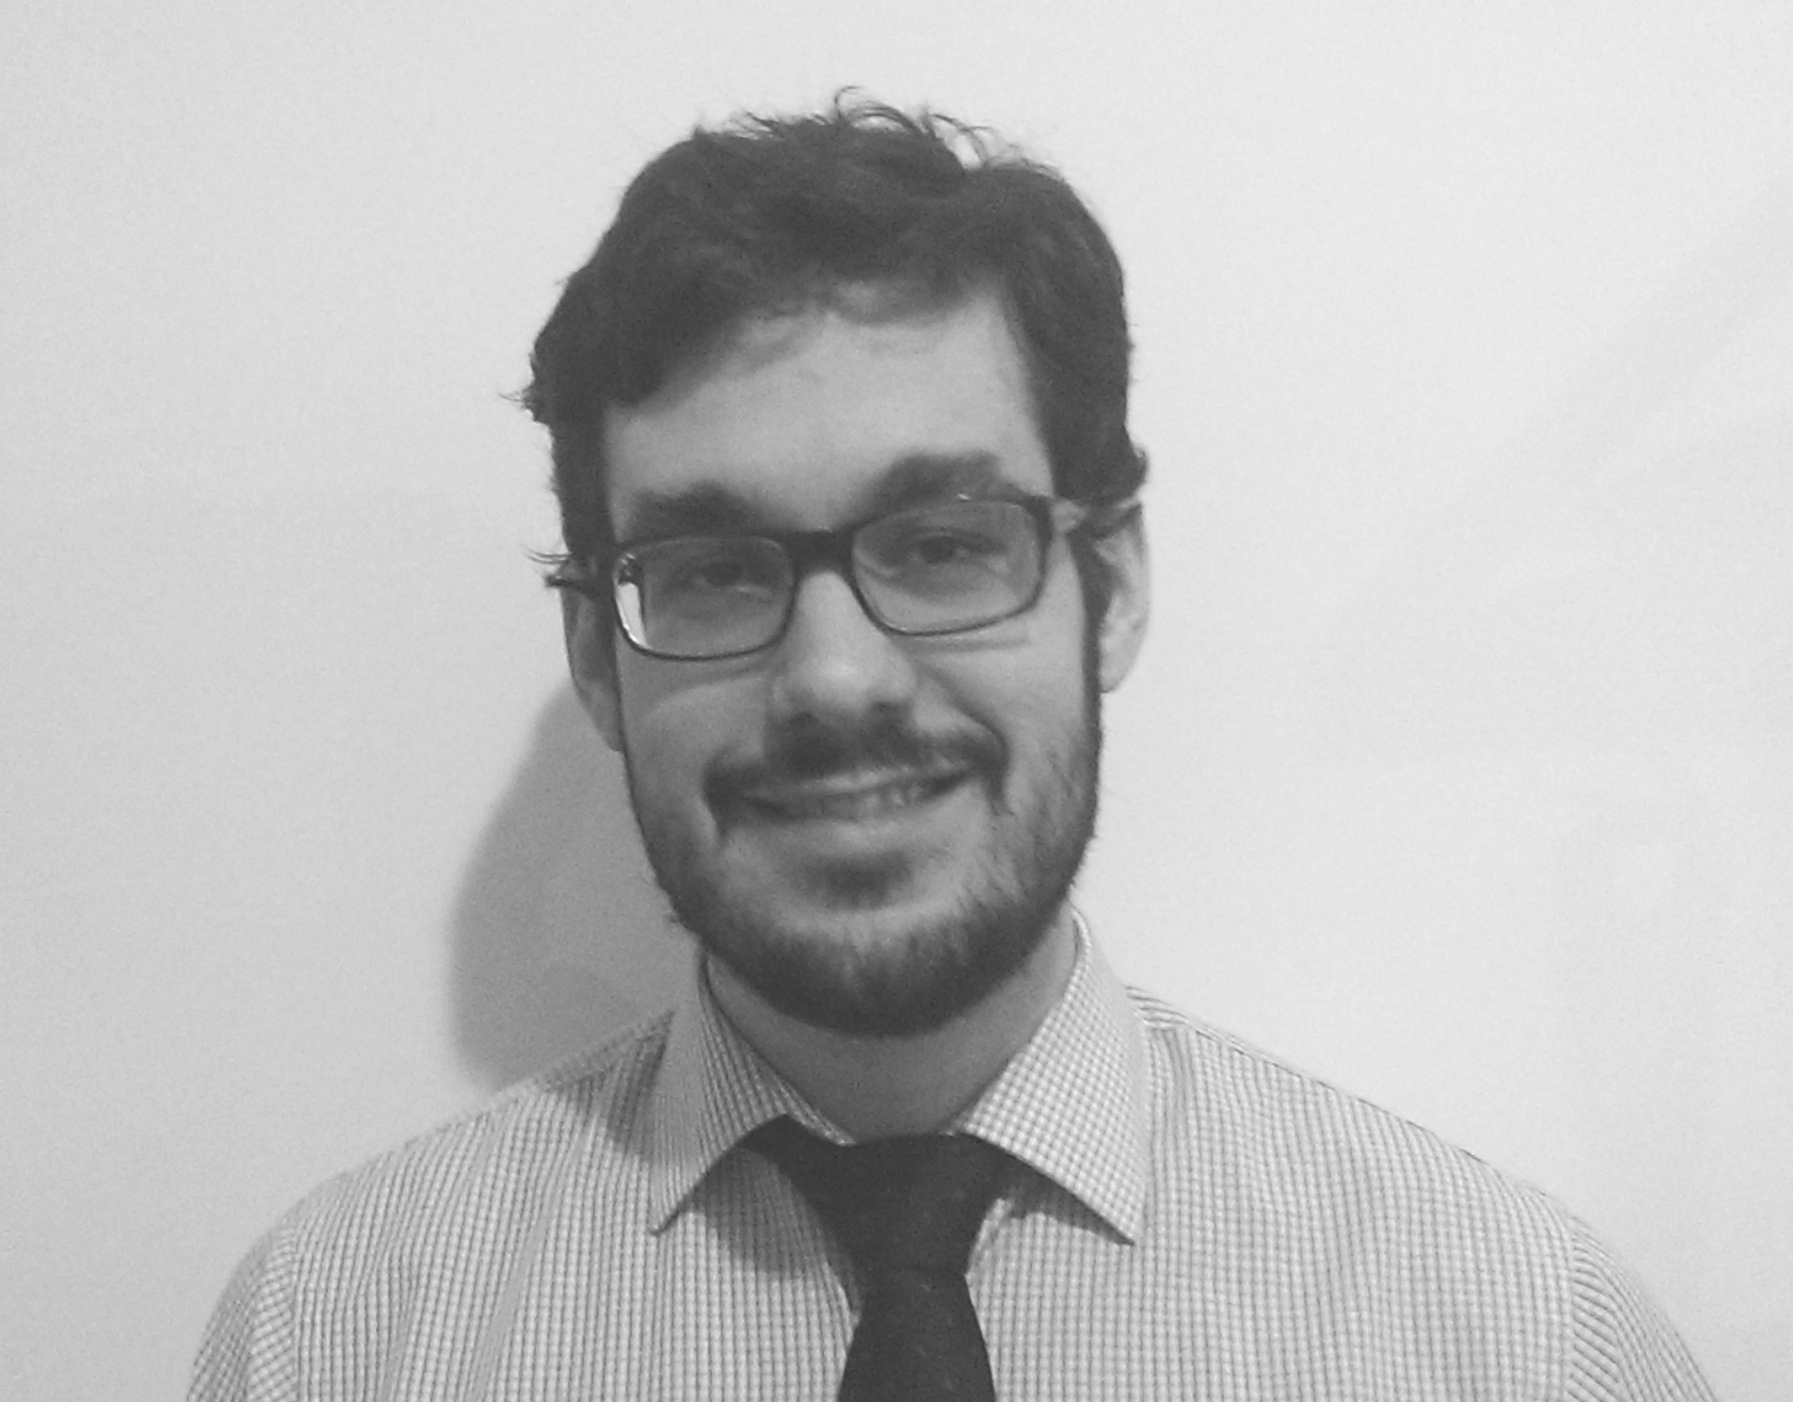
\includegraphics[width=2in,height=2.5in,clip,keepaspectratio]{nik_headshot}
%\end{wrapfigure}

Nik did some physics. It could have gone much better; he's not sure how. 

\end{vita}
\end{document}
